
\chapter{Marco teórico}

\label{ch:background}

\section{Consideraciones previas}
En general durante el presente trabajo, para estudiar la estabilidad de los puntos de equilibrio de una ecuación diferencial autónoma, sea cual sea el sistema, hemos recurrido a la linearización del modelo en torno a ellos. Tenemos asegurado que podemos estudiar localmente esta característica gracias al \textbf{teorema de Hartman-Grobman}:
\begin{theorem}
	Consideremos un sistema de la forma $x'=f(x)$ para alguna $f: \mathbb{R}^n \to \mathbb{R}^n$ suficientemente derivable.
	Supongamos que el sistema tiene un estado hiperbólico de equilibrio: $x^*\in\mathbb R^n$: esto es, $f(x^*)=0$ y la matriz Jacobiana de $f$ en $x^*$ no tiene valores propios con parte real igual a 0.\\ Entonces existe un entorno $\Omega$ del equilibrio $x^*$ y un homeomorfismo $h : N \to \mathbb{R}^n$,
	de manera que  $h(x^*)=0$
	y en este entorno $\Omega$ el comportamiento de $x'=f(x)$ es topológicamente equivalente por $X=h(x)$ al comportamiento del sistema linearizado $dX/dt=AX$, donde $A$ corresponde a la matriz Jacobiana de $f$. 
	\end{theorem}

Este teorema es ampliamente utilizado y su demostración puede encontrarse, por ejemplo en \cite{perko}, en la que sigue una filosofía constructiva. Por otra parte puede que al lector no le resulte familiar el concepto de topológicamente equivalente. En ese caso puede consultar la \emph{Definición} \ref{topequi} sobre \emph{equivalencia topológica}.

\section{Órbitas y ciclos límite}
A poco que nos adentremos en sistemas de dos dimensiones podremos comprobar cómo afloran una serie de comportamientos cualitativos íntimamente relacionados con las órbitas cerradas. Dado que conceptos como órbita cerrada o ciclo límite nos serán de importancia a la hora de describir una de las bifurcaciones más importantes en dimensión 2, es indispensable introducir aquí esos conceptos así como resultados teóricos que los fundamenten cuando nos encontremos este comportamiento.
Introducimos  la notación que usaremos durante este apartado, así como el marco teórico de referencia:\\
Sea $D$ un subconjunto abierto de $\mathbb{R}^2$ y sea $F=(f_1,f_2):D\subseteq \mathbb{R}^2 \rightarrow \mathbb{R}^2 $ una función continua, que nos define el siguiente sistema autónomo:

\begin{equation} \left \{ \begin{matrix} x_1'=f_1(x_1,x_2)\\ x_2'=f_1(x_1,x_2).  \end{matrix}  \right.\label{sist}\end{equation}
Asumiremos que el sistema está en las condiciones para aplicar el teorema de existencia y unicidad para tiempo $t_0$ con condiciones $x_1(t_0) , x_2(t_0)$ y llamaremos a la solución $\phi(t)=(\phi_1(t),\phi_2(t))$.

 Basándonos en la definición de órbita estudiada en la asignatura de ecuaciones diferenciales II, que recuperamos para una mejor comprensión, introducimos los primeros conceptos:
  \begin{defi}[Órbita]
  	Dado un sistema de ecuaciones (\ref{sist}), llamamos órbita al conjunto de puntos:  $P(t)=(\phi_1(t),\phi_2(t))$, 
  	con $t\in \mathbb{R}$  .
  \end{defi}
  
 \begin{defi}[Semiórbita]
 	Dada una órbita $C$, definimos una \textbf{semiórbita positiva} $C^+$ (respectivamente negativa como $C^-$) desde $t_0$ como el conjunto $P(t)=(\phi_1(t),\phi_2(t))$ de todos los puntos de $D$ donde \(t_0\leq t < \infty\) (respectivamente \(-\infty< t < t_0\)).
 \end{defi}
 Dentro de este conjunto definiremos los puntos límite, que serán fundamentales para la creación de este cuerpo teórico:
 \begin{defi}[Punto límite]
 	
 	Dada una semiórbita $C^+$(respectivamente $C^-$), decimos que un punto $Q$ en el plano \((x_1,x_2)\) es un \textbf{punto límite} si existe una sucesion de números reales \( \{t_n\}, n\in \mathbb{N}\) tal que si $n\rightarrow \infty$ entonces $t_n\rightarrow \infty$ y $P(t_n)\rightarrow Q$ .
 \end{defi}
 \begin{defi}[Conjunto límite]
 	
 	Denotamos por\textbf{ conjunto límite}, $L(C^+)$(respectivamente $L(C^-)$), al conjunto de todos los puntos límite de una semiórbita $C^+$(respectivamente $C^-$).
 \end{defi}
 Antes de seguir, vale la pena añadir que en el caso en el que consideremos una órbita completa, $C$, las definiciones anteriores tienen perfecto sentido y pueden notarse sustituyendo $C^+$ por $C$. Además, es completamente trivial definir el conjunto límite a través de la unión de los conjuntos límites de las semiórbitas asociadas.\\
 
 Una vez tenemos ya la notación básica, podemos pararnos a reflexionar sobre la naturaleza del mismo, para que intuitivamente afloren las restricciones que realizaremos. Como comentábamos, nuestra idea es explorar la existencia de comportamientos periódicos, que vienen asociados con una trayectoria cerrada (curva simple cerrada).
 
  Si bien esto no es la tónica general que podemos encontrar en nuestros planos de fase, es cierto que a poco que pensemos en la naturaleza de esta órbita, es inmediato razonar que nos restringiremos al estudio de conjuntos compactos dentro de nuestro dominio D, nótese que de otra manera nada nos garantiza que haya órbitas periódicas que estudiar. Es natural preguntarse si, aún con nuestra restricción, podemos encontrar estas órbitas, para ello, recurrimos al siguiente resultado:
 \begin{theorem}[]
 	Si $C^+$ es un semiórbita positiva contenida en un subconjunto compacto K de D, entonces $L(C^+)$ es un conjunto no-vacío, compacto y conexo.
 	\begin{proof}
 		Primero probaremos que el conjunto $L(C^+)$ es no vacío y está contenido en K, desde ahí probaremos que es cerrado, acabando con la demostración de la conexión por reducción al absurdo.
 		Sea $C^+$ una semiórbita contenida en un compacto $K$, podemos tomar una sucesión de puntos definida como $\{P_n\}=\{(\phi_1(t_0+n),\phi_2(t_0+n))\} \forall n \in \mathbb{N}$. Como esta sucesión está contenida en un conjunto acotado, en particular, tendrá una parcial convergente. Además, como es compacto, el punto al que converja debe estar dentro de K, luego $L(C^+)$ no será vacío y $L(C^+) \subseteq K$.
 		
 		El siguiente paso será probar que el conjunto límite es cerrado.
 		Sea $R$ un punto de acumulación del conjunto $L(C^+)$, por definición, existe una sucesión $\{R_n\}_{n\in\mathbb{N}}$ de elementos del conjunto límite de manera que la distancia entre $R$ y $R_n$ tiende a cero cuando $n\to \infty$. Para cada $R_n$ existirá un término a partir del cual la distancia sea menor que 1/n. Por tanto para cualquier $\epsilon >0$ existirá  $m_\epsilon$ tal que $\forall n>m_\epsilon$, $ dist((\phi_1(t_n),\phi_2(t_n)),R_n)<\epsilon/2$ y $dist(R_n,R)<\epsilon/2$. Esto implica que para $n>m_\epsilon$, $ dist(\phi_1(t_n),\phi_2(t_n)),R)<\epsilon$. Concluyendo que $R\in L(C^+)$ y por tanto, el conjunto $L(C^+)$ es cerrado.
 		
 		Supongamos ahora que $L(C^+)$ no es conexo y que existen dos conjuntos conexos, cerrados y disjuntos $A , B$ cuya unión es nuestro conjunto límite. Como ambos son acotados existirá una distancia finita entre ellos: $\delta$. Por otra parte como los puntos de $A$ y $B$ pertenecen al conjunto límite,lo que implica que existirá un $t$ arbitrariamente grande de manera que el conjunto de los puntos límite ($P(t)$) diste de $B$ una distancia menor de $\delta /2$, y otro $t$ arbitrariamente grande de manera que $P(t)$ diste más de $\delta /2$. Como la distancia entre el conjunto de puntos y $B$ es una función continua y, recordemos que está formado por $\phi_1$ y $\phi_2$, también continuas, no queda más remedio que admitir que existe una sucesión ${t_n}$ de manera que la distancia entre $P(t_n)$ y $B$ sea $\delta/2$ con $t_n\rightarrow \infty$ cuando $n\rightarrow \infty$. Esa sucesión debe contener, por el mismo motivo que el primer párrafo de la demostración, una parcial convergente a un punto $Q$. Por tanto $Q \in L(C^+)$ y $dist(Q,B)=\delta/2$. Pero esto implica que $Q$ no está ni en $A$ ni en $B$ puesto que: $dist(Q,A)\geq dist(A,B)-dist(Q,B)=\delta/2$, lo que resulta en contradicción puesto que por hipótesis $L(C^+)=A\cup B$.
 	\end{proof}
 \end{theorem}
 Siendo este el principal resultado podemos añadir como corolario:
 \begin{corollary}
 	Sea $C^+$ en las condiciones del teorema anterior. Si existe $Q\in L(C^+)$ de manera que Q no es un punto fijo (es decir, f1, f2 no se anulan), entonces la órbita que pasa por el punto $Q$,$C_Q$, existe como una órbita completa y $C_Q\subseteq (C^+)$.
 \end{corollary}
 Este resultado que se desprende del anterior teorema, añadiendo la dependencia continua de la solución respecto  los valores iniciales, nos da pie a nombrar $C_Q$ como: \textbf{órbita límite\footnote{Nótese que no hemos comentado nada sobre los posibles puntos críticos o puntos fijos de $F$, por lo que sabemos hasta ahora el objeto que definimos como conjunto límite, está formado por ellos o por órbitas límite.} de $C^+$}.
 
 \subsection{Teorema de Poincaré Bendixson}
 Si hemos de remarcar algún resultado en esta sección, ese debe ser, sin ninguna duda, el teorema de Poincaré Bendixson. Este teorema es el eje principal alrededor del cual giran otros muchos resultados en lo que al estudio de sistema dinámicos 2-dimensionales se refiere. Además, de su demostración se sigue singularmente una propiedad que comentaremos al final del apartado: la inviabilidad de la obtención de teoremas similares en dimensión superior a 2.
 La prueba aquí expuesta está basada en la dada por Coddintong-Levyson\cite{codin}. Aunque un tanto larga, la demostración requiere de ideas y conceptos interesantes que suponen un añadido al conjunto de herramientas con las que atacar demostraciones de índole similar, es por eso que he elegido esta y no otra.
 \begin{theorem}[Poincaré Bendixson]
 	\label{Poincare-Bendixson}
 	Sea $C^+$ una semiórbita positiva contenida en un subconjunto cerrado $K$ de $D$. Si $L(C^+)$ esta formado únicamente por puntos regulares entonces se da alguna de las siguientes situaciones:
 	\begin{itemize}
 		\item $C^+(=L(C^+))$ es una órbita periódica
 		\item $L(C^+)$ es una órbita periódica
 	\end{itemize}
 	Es decir, o nuestra solución se acercará indefinidamente a una órbita periódica o será una órbita periódica.
 \end{theorem}
 Con el fin de demostrar el teorema exitosamente debemos introducir previamente un concepto.\\
 \begin{defi}[Transversal]
 	Un segmento cerrado y finito $l$ de una línea recta en el plano $(x_1,x_2)$ será denominado \textbf{transversal} con respecto a una función $f$ si todo punto de $l$ es regular y la dirección determinada por $f$ en todo punto de $l$ es diferente a la determinada por $l$.
 \end{defi}
 \begin{figure}[h]
 	\centering
 	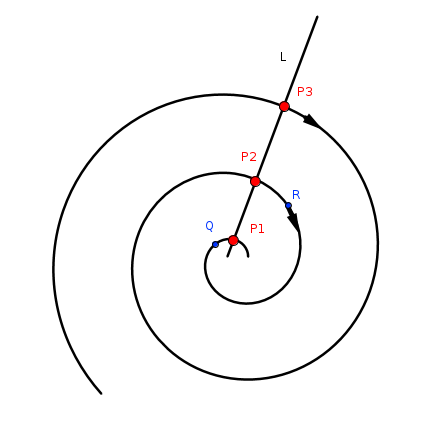
\includegraphics[width=0.5\textwidth]{transversal.png}
 	\caption{Ejemplo de transversal L.   }
 	\label{transversal}
 \end{figure}
 Usando el concepto recién definido utilizaremos cuatro lemas, que allanarán la demostración que perseguimos. Únicamente demostraremos los lemas \ref{lema1} y \ref{lema2} que son los utilizados directamente en el teorema y también son piedra angular de las pruebas de los múltiples corolarios que se pueden obtener:
 \begin{lemma}
 	\begin{enumerate}[i.]
 		\item Todo punto regular de D es un punto interior de alguna transversal, que tendrá cualquier dirección excepto la de la transversal
 		\item Toda órbita que se encuentre con una transversal debe cruzarla y todas estas órbitas la cruzarán en la misma dirección
 		\item Sea $P_0 \in D $ un punto interior de una transversal l. Para todo $\epsilon>0$ existe  un círculo $C_\epsilon$ con $P_0$ como centro tal que toda órbita que pasa por un  punto del interior de $C_\epsilon$ para $t=0$ cruza $l$ para algún $t, |t|< \epsilon$ 
 	\end{enumerate}
 \end{lemma}
 \begin{lemma}
 	Si un arco finito cerrado $A$ de una órbita C interseca una tranversal, lo hace en un conjunto finito de puntos, cuyo orden (o cantidad de puntos) en $A$ es el mismo que el orden en $l$. Si $C$ es una órbita periódica, sólo interseca a la tranversal en un punto.
 \end{lemma}
 \begin{lemma}
 	Si $C^+$ y $L(C^+)$ tienen un punto en común entonces $C^+$ es una órbita periódica.
 	\label{lema1}
 \end{lemma}
 \begin{proof} \textbf{Lema \ref{lema1}}.\\ 
 	Sea $P_1=P(t_1)$ un punto de $C^+$ que a su vez pertenezca a $L(C^+)$. Es un punto regular por lo que también es un punto interior de nuestra transversal $l$. Como $P_1 \in L(C^+)$ cualquier círculo $\Gamma$ con $P_1$ como centro, debe contener en su interior un punto $Q=P(t_k), t_k>t_1+2$. Si $\Gamma$ es el círculo para $\epsilon=1$ en el lema 2.2.3 (III), entonces existe $P_m=P(t_m)$ donde $|t_k-t_m|<1$ y $P_m$ está en $l$. Si $P_m$ es distinto de $P_1$ entonces el arco $P_1P_m$ de $C^+$ interseca a $l$ en un número finito de puntos por el lema 2.2.4. Además las intersecciones sucesivas de $C^+$ con $l$ forman una secuencia monótona que tiende a alejarse de $P_1$. Por tanto $P_1$ no puede ser un punto límite de $C^+$ (y por ende, no está en $L(C^+)$). La consecuencia es que $C^+$ solo cruza a $l$ en $P_1$, lo que implica que $C^+$ es una órbita periódica.
 \end{proof}
 \begin{lemma}
 	Si $L(C^+)$ contiene una órbita periódica entonces es idéntica a ella.
 	\label{lema2}
 \end{lemma}
 \begin{proof}\textbf{Lema \ref{lema2}}.\\
 	Sea $C_0$ una órbita periódica en $L(C^+)$ y supongamos que está contenida en $L(C^+)$. Entonces, como $L(C^+)$ es conexo, $C_0$ contiene un punto de acumulación $Q_0$ del conjunto $L(C^+)-Q_0$. Sea ahora la transversal $l$ que pasa por $Q_0$, entonces todo círculo que tenga por centro a $Q_0$ contiene un punto $Q$ de $L(C^+)-C_0$, y, para $Q$ suficientemente cercano a $Q_0$, la órbita $C_Q$ sobre $Q$ cortará a la transversal por el lema 2.2.3(III). La órbita $C_Q$, es una órbita límite por el corolario 1.1 y es distinta de $C_0$ puesto que se verifica que $C_Q\subseteq L(C^+)-C_0$. Por tanto $l$ contiene dos puntos distintos de $L(C^+)$, lo cual contradice el lema anterior. La contradicción viene de suponer que la órbita periódica está estrictamente contenida en $L(C^+)$, con lo que demostramos el resultado.
 \end{proof}
 Concluidos los lemas previos, obtenemos la demostración del teorema de Poincaré Bendixson:
 \begin{proof}
 	Claramente si $C^+$  es una órbita periódica entonces $C^+=L(C^+)$ . Por tanto asumimos de aquí en adelante que $C^+$  no es periódica. Como $L(C^+)$ no es vacío  y consiste solo en puntos regulares existe por el teorema 2.2 una órbita límite $C_0$ en $L(C^+)$. Ahora, dado que $C_0\subseteq K$, esto implica que la semiórbita $C_0^+$ tiene un punto límite $P_0$ y $P_0 \in L(C^+)$, para $L(C^+)$ cerrado. Si l es una transversal por $P_0$, entonces, dado que $P_0$ y $C_0^+$ están ambas en $L(C^+)$, la transversal l solo puede cruzar $L(C^+)$ por $P_0$ ( por el lema 2.2.3). Teniendo en cuenta que $P_0$ es un punto límite de $C_0^+$, l debe intersecar $C_0^+$ en algún punto, que debe ser $P_0$ y por tanto, $C_0^+$ y $L(C^+)$ tienen un punto en común: $P_0$. Por el lema 2.2.5 $C_0^+$ (y en consecuencia $C_0$), son órbitas periódicas, y esto implica, por el lema 2.2.6, que $C_0=L(C^+)$
 \end{proof}
 
 \begin{corollary}
 	Si $C^+$ es una semiórbita contenida en un compacto K el cual no posee puntos críticos, entonces K contiene una órbita periódica.
 \end{corollary}
 
 
 Podemos alargar el resultado un poco más, añadiendo el caso en el que nos encontremos con un número finito de puntos críticos.
 
 \begin{theorem}
 	Sea $C^+$ una semiórbita contenida en un subconjunto compacto K de D y suponiendo que D tenga un número finito de puntos críticos. Entonces se pueden dar tres situaciones (excluyentes):
 	\begin{enumerate}
 		\item $L(C^+)$ consiste en un único punto crítico de F al cual se aproxima $C^+$ cuando $t\leq \infty$,
 		\item $L(C^+)$ es una órbita periódica,
 		\item $L(C^+)$ consiste en un conjunto finito de puntos críticos de F y un conjunto de órbitas, cada una de las cuales tiende a cada uno de los puntos críticos.
 	\end{enumerate}
 \end{theorem}

\subsection{Otros criterios útiles}
Mostramos en este apartado cómo el teorema de Poincaré Bendixon es bastante singular en su campo. Tenemos frente a él multitud de criterios para eliminar la existencia de órbitas cerradas. Presentamos, para ilustrar este comentario dos ejemplos también muy útiles.
\subsubsection{Criterio de Dulac}
\begin{theorem}
	Sea $(x_1,x_2)'=f(x_1,x_2)$ un campo de vectores definido en un subconjunto conexo $R$ del plano de componentes $(f_1(x_1,x_2), f_2(x_1,x_2))$. Si existe una función real de variable real, continuamente diferenciable $g(x_1,x_2)$ tal que $\nabla(g.f)) $ tiene signo constante distinto de $0$  en $R$, entonces $R$ no puede albergar ninguna órbita cerrada completa.
\end{theorem}
\begin{proof}
Sin perder generalidad, supongamos que existe una función $g(x_1,x_2)$ de manera que \[ \frac { \partial (g.f_1) }{ \partial x_1 } +\frac { \partial (f_2.g) }{ \partial x_2 } >0, \]
en una región simplemente conexa $R$. Sea $C$ una órbita cerrada de nuestro sistema autónomo en $R$. Sea $D$ el interior de C, que sabemos que existe por el teorema de la curva de Jordan: Toda curva cerrada simple del plano divide al plano en dos componentes conexas disjuntas que tienen a la curva como frontera común. Una de estas componentes está acotada (el interior de la curva) y la otra es no acotada y se le llama exterior\footnote{Para la demostración de este teorema, consúltese: \cite{jordan}}. Entonces, aplicamos el teorema de Green: 
\begin{align}
 \iint _{ D }^{  }{ \frac { \partial (g.f_1) }{ \partial x_1 } +\frac { \partial (f_2.g) }{ \partial x_2 } dx_1dx_2 } =\oint _{ C }^{  }{\left( -g f_2dx_1+g f_1 dx_2 \right)}= \\
= \oint _{ C }^{  }{ g \left( - x_2' dx_1+x_1' dx_2 \right)  }.
\end{align}
Pero en $C$ $dx_1=x_1'dt$ y $dx_2=x_2'dt$ por lo que la integral (2.3) es $0$. Con ello llegamos a contradicción puesto que en la primera integral de (2.2), $D$ es un área no nula y el integrando es una función cuyo signo no cambia. Esto implica que esa integral no podría ser 0, lo que nos lleva a contradicción. Por tanto no puede existir esta órbita cerrada $C$. 
\end{proof}
Más información sobre la prueba y corolarios se pueden encontrar en \cite{dulac}.

\subsubsection{Criterio del gradiente}
Decimos que nuestro sistema es un sistema conservativo o gradiente si puede ser escrito de la forma:
\begin{equation}
x'=-\nabla V.
\label{gradiente}
\end{equation}
donde V es una función escalar continuamente diferenciable llamada potencial.
\begin{theorem}
En sistemas conservativos no pueden existir órbitas cerradas.
\end{theorem}
\begin{proof}
	Supongamos lo contrario. Obtendremos contradicción considerando la evolución de V a lo largo de un ciclo de periodo $T$. 
	Por una parte, tenemos que $V(T)-V(0)=0$ por hipótesis. Pero, por otra parte
	\[ V(T)-V(0)=\int_{0}^{T}\frac{dV}{dt}dt=
	\int_{0}^{T}\nabla V\cdot x'dt=
	\int_{0}^{T}-||x'^2||<0. \]
	(Obviamos el caso $x'=0$ pues en ese caso tendríamos un punto fijo, no una órbita). Llegamos por tanto a contradicción, no pueden existir órbitas cerradas.
\end{proof}


\section{Osciladores fisiológicos}
Para mostrar una aplicación directa del teorema de Poincaré Bendixson, vamos a tratar un modelo conocido como oscilador de \textit{ Van der Pol}.

Si bien el nombre es puramente intuitivo, a modo de aclaración, estamos ante la descripción de un sistema que experimenta o es capaz de crear perturbaciones o cambios periódicos en un medio.
Este oscilador fue descrito originalmente por Balthasar Van der Pol \cite{vander} debido al descubrimiento de lo que el denominó \textit{oscilaciones de relajación}, en circuitos que usaban válvulas de vacío. Pudiera parecer que estamos ante un nuevo concepto, pero estas oscilaciones corresponden a nuestra definición de conjuntos límite, matizando que nos referimos al caso de órbitas cerradas.

Aunque la aparición de este concepto está alejada de ámbitos biológicos, no tardaron en aparecer aplicaciones al campo de la neurociencia. La primera de ellas corresponde a los trabajos de Fithugh y Nagumo donde aplicaron el modelo sobre un campo bidimensional para describir el potencial de acción de las neuronas \cite{fit, nagu}. No sólo la neurociencia se vio alumbrada bajo este nuevo modelo, en \cite{mathmobi} podemos encontrar como esas ecuaciones también se usaron para describir otros procesos fisiológicos como las oscilaciones de los latidos del corazón.

\begin{equation}
x''-\alpha(1-x^2)x'+x=0,\text{ } (\alpha>0).
\label{vanderpol}
\end{equation}

En estas condiciones, fijando el parámetro como $\alpha=1$ vamos a realizar un cambio de variable para disponer del sistema de una forma más operable:
\begin{equation}
y=x-\frac{x^3}{3}-\frac{x'}{1}.
\label{cambio}
\end{equation}
De donde:
\begin{equation}
x'=(x-\frac{x^3}{3}-y).
\end{equation}
Derivo (\ref{cambio}), 
\begin{equation}
y'=x'(1-x^2)-\frac{x''}{1}.
\label{77}
\end{equation}
De (\ref{vanderpol}) tenemos:
\begin{equation}
\frac{x}{1}=-\frac{x''}{1}+(1-x^2)x'
\label{99}
\end{equation}
Igualando (\ref{77}) y (\ref{99}) nos queda esta representación:
\begin{equation}
 \left \{ \begin{matrix}x'=-y-x^3/3+x  \\y'=x\end{matrix}\right.. 
\label{vanderpol2}
\end{equation}
Acto seguido calculamos las nulclina de nuestro sistema, que igualando a $0$ cada una de las ecuaciones nos llevan a afirmar que estas vienen dadas por las curvas:
\begin{equation}
 \left \{ \begin{matrix}y=x^3/3+x \text{ (la nulclina asociada a x)}  \\x=0 \text{ ( la nulclina asociada a y)}\end{matrix}\right.. 
\label{nulclinas}
\end{equation}
Sale aquí de manifiesto el porqué este problema también es conocido como el de la nulclina cúbica. De hecho, como veremos en el comportamiento cualitativo, todas las características de nuestro modelo sencillo nos llevan indudablemente a una rápida aplicación del teorema.
De (\ref{nulclinas}) podemos observar el siguiente comportamiento de los vectores de dirección de nuestras soluciones, teniendo en cuenta (\ref{vanderpol2}):
\begin{figure}[h]
	\centering
	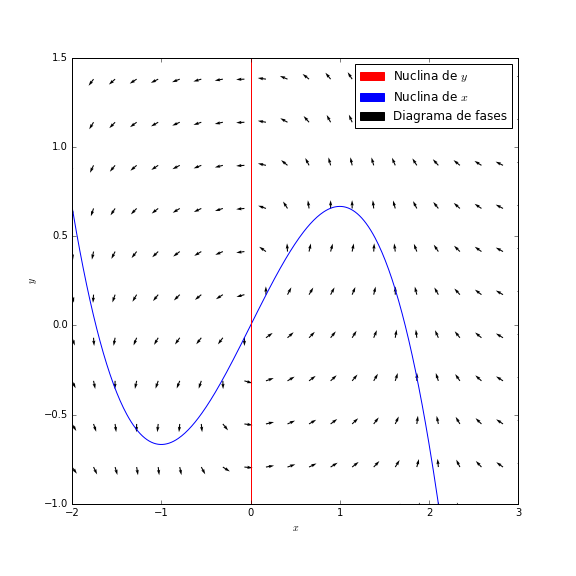
\includegraphics[width=0.5\textwidth]{phasefinal.png}
	\caption{Diagrama de fase de nuestro oscilador. Se puede observar la aparición del ciclo límite  }
\label{poincaa}
\end{figure}
\begin{itemize}
	\item La dirección debe ser \textquotedblleft vertical\textquotedblright en la nulclina de $x$ y \textquotedblleft horizontal\textquotedblright en la de $y$ (ya que $x' = 0$ o $y' = 0$, respectivamente).
	\item Cuando x es positivo, $y$ disminuye.
	\item  En la nulclina de $y$, $x$ es cero de modo que $x^3/3-x$ es también cero. Así por (\ref{vanderpol2}) $x'=y$, y $x$ aumentará cuando $y$ sea positiva y disminuirá cuando $y$ sea negativa.
\end{itemize}
Consideremos ahora una trayectoria que emana de un punto arbitrario en el primer cuadrante (el positivo). El flujo en la proximidad del nulclina de $x$ lo llevará a través de una disminución de valores de $x$. Después de llegar al segundo cuadrante y cerca del mínimo local de la nulclina, el flujo se desvía horizontalmente a través de y, hacia la rama izquierda de la curva cúbica.
Aquí una corriente en la dirección y positiva llevaría la solución desde el tercer cuadrante, de nuevo al primero como se observa en la Figura (\ref{vande}).\\
\begin{figure}[h]
	\centering
	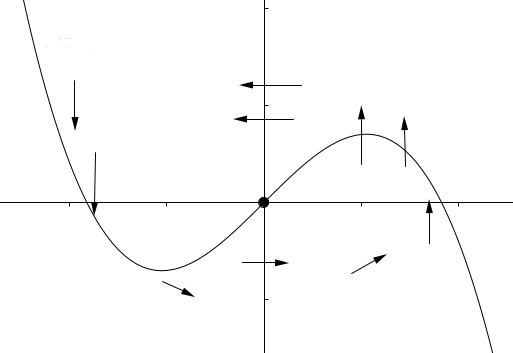
\includegraphics[width=0.5\textwidth]{vande.png}
	\caption{Diagrama de los vectores alrededor de la nulclina según el estudio.  }
	\label{vande}
\end{figure}

Concluida esta observación es evidente, además, que la solución permanecerá dentro o paralela a una región acotada, indicando que una vez que una trayectoria ha entrado en la región, está atrapada para siempre. 

En esta región además, hay un punto fijo: $(0,0)$.
Si calculamos la matriz Jacobiana para estudiar su estabilidad, obtenemos:
\[ J= \begin{pmatrix} 1-x^2 & -1 \\ 1 & 0 \end{pmatrix} .\]
Por lo que evaluando en $(0,0)$ obtenemos $Traza(J(0,0))=1$ y $Det(J(0,0))=1$. Tenemos espirales que repelen, es decir, un punto inestable.\\
Por lo tanto podemos aplicar el teorema de Poincaré-Bendixson concluyendo que hay un ciclo límite dentro de esta región. \\
Este oscilador ha sido además utilizado en otras áreas como la neurociencia. Ayudándose del mismo Tizhugh y Nagumo (como se puede ver en \cite{mathmobi}), aplicaron los conceptos subyacentes para estudiar el potencial acción de las neuronas.

En análisis de posteriores casos de este trabajo, se usará también este teorema para detectar la existencia de órbitas periódicas.
 
 
 
 \section{Conceptos Básicos de teoría de Bifurcaciones}
 La teoría de bifurcaciones es una rama de estudio relativamente reciente. Adquiere verdadera importancia  a partir de un artículo famoso de E.Hopf publicado en 1942, donde se relaciona la aparición de soluciones periódicas con ciertos cambios en el comportamiento de la parte lineal del sistema tras un cambio de un parámetro.\\
 Antes de formalizar el concepto, nos adentramos en esta teoría a través de una definición que, si bien no es estrictamente rigurosa, nos sirve para captar el concepto rápidamente gracias a nuestros conocimientos acerca de la noción de estabilidad que obtenemos en la asignatura Ecuaciones Diferenciales II: 
 \begin{defi}[Bifurcación (Intuitiva)]
 	Una bifurcación en un sistema dinámico no es mas que un cambio cualitativo en el diagrama de fases de nuestro sistema originado por la variación de uno o varios de los parámetros que en él se encuentran (mas concretamente cuando este parámetro alcanza o sobrepasa un valor crítico).
 \end{defi}
 Entendida la idea intuitiva pasamos a formalizar el concepto. He querido partir de una base sólida para no dar por sentado aspectos que pudieran pasarse por alto. Es por eso que comienzo desde la raíz topológica de esta rama.
 Si queremos estudiar las diferencias entre características cualitativas de los sistemas dinámicos, debemos razonar que este estudio pasará inexorablemente por clasificar los tipos de comportamientos que podemos observar en nuestros sistemas y compararlos entre sí. Para ello se hace indispensable la creación de una relación de equivalencia rigurosamente definida que nos permita decidir cuando dos sistemas dinámicos (o un conjunto de $n \in \mathbb{N}$ ) son cualitativamente similares o equivalentes:
 \begin{defi}[Equivalencia topológica entre dos sistemas dinámicos]
 	Un sistema dinámico $ \{T, \mathbb{R}^n , \phi(t) \}$ es considerado topológicamente equivalente o equivalente a un sistema dinámico $ \{T, \mathbb{R}^n , \psi(t) \}$ si existe un homeomorfismo $h : \mathbb{R}^n \rightarrow \mathbb{R}^n$ que lleva las órbitas del primero en las de el segundo, preservando la dirección del tiempo.
 	\label{topequi}
 \end{defi}
 Entiéndase que $T$ puede ser una variable temporal tanto continua como discreta. Además podemos considerar otros espacios de $\mathbb{R}^n$ para los que nuestra definición también sería correcta y útil, por ejemplo el toro o la esfera.
 Sin embargo, dado que la mayoría de modelos a estudiar estarán planteados en $\mathbb{R}$ o $\mathbb{R}^2$ , trabajaremos con ellos, de aquí en adelante.
 Tenemos ya todas las herramientas para definir correctamente el objeto de nuestro estudio: \\
 
 Sea el sistema dinámico definido por: 
 \begin{equation}
 x'=f(x,\alpha)
 \label{defi1}
 \end{equation}
 donde $x \in \mathbb{R}^n$ corresponde a nuestras variables y $\alpha \in \mathbb{R}^n$ corresponde a los parámetros que aparecen en nuestro sistema.
 \begin{defi}[Bifurcación (formal)]
 	La aparición de un diagrama de fases de \ref{defi1} no equivalente topológicamente bajo la variación de $\alpha$ es lo que denominamos bifurcación.
 \end{defi}
 
 Antes de pasar a la clasificación de una variada cantidad de bifurcaciones nos queda definir una forma estándar, no tanto un representante de cada una de las clases de equivalencia, si no más bien una forma de encontrar a éste:
 
 \begin{defi}[Forma Normal]
 	Diremos que un sistema de la forma: 
 	\begin{equation}
 	\xi'=f(\xi,\beta)
 	\end{equation}
 	donde $f$ es de forma polinomial con un punto de equilibro en $\xi=0$ cuando $\alpha=0$, es la forma normal de \ref{defi1} si son localmente topológicamente equivalentes en un entorno del equilibrio cuando $x=0$ y $\alpha=0$.
 \end{defi}
 
 Y, por último, durante nuestro estudio utilizaremos una representación visual de las bifurcaciones, lo que conocemos por un diagrama de bifurcaciones:
 \begin{defi}[Diagrama de Bifurcaciones]
 	Un diagrama de bifurcaciones de $(2.1)$ no es mas que una representación gráfica que enfrenta a nuestra variable x con el valor de nuestro parámetros y delimita las zonas agrupando las soluciones que son topológicamente equivalentes. 
 \end{defi}
 
 \subsection{Clasificación de las principales bifurcaciones en sistemas \\  1-dimensionales y 2-dimensionales}
 
 \subsubsection{Sistemas 1-dimensionales}
 
 \begin{enumerate}
 	\item Bifurcación Saddle Node o Fold\\
 	Esta bifurcación es el mecanismo básico mediante el cual, a través de la variación del parámetro aparecen y colisionan\footnote{el término colisión no es casual, basta comprobar que, sea $v(\alpha)$ la velocidad de aproximación de los puntos fijos $\Rightarrow$ $v(\alpha) \rightarrow \infty $ cuando $\alpha \rightarrow 0$} puntos fijos. 
 	La forma normal de esta bifurcación es:
 	\begin{equation}
 	x'=\alpha+x^2
 	\label{sadd}
 	\end{equation}
 	donde $\alpha$ es un parámetro que puede ser positivo, negativo o 0.
 	Para estudiar de manera óptima como cambia nuestra solución discutiremos la variación en una partición de $\mathbb{R}$:\\
 
 	\begin{itemize}
 		\item $\alpha \in \mathbb{R^-} $ : en este caso el signo de la derivada cambia cuando x=0 por lo que tendremos la existencia de dos puntos fijos $x_{1,2}(\alpha)=\pm \sqrt{-\alpha}$: uno estable puesto que la derivada será positiva $\forall x \in \mathbb{R},\text{ } x < x_1$ y negativa $\forall x \in \mathbb{R},\text{ } x_1< x < x_2$. Otro inestable, puesto que los signos de la derivada varían de forma opuesta: negativa para $\forall x \in \mathbb{R},\text{ } x_1 <x < x_2$ y positiva para $\forall x \in \mathbb{R},\text{ } x_2 < x$
 	\begin{figure}[h]
 		\centering
 		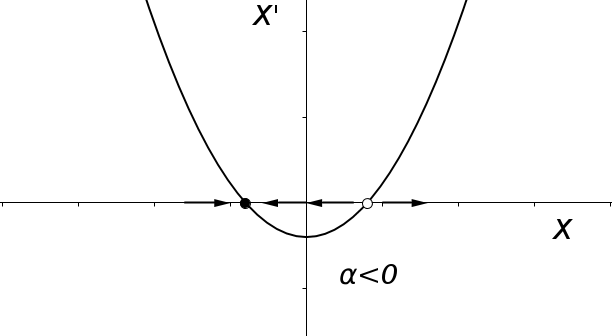
\includegraphics[width=0.5\textwidth]{saddlenode3.png}
 		\caption{Comportamiento de (\ref{sadd}) con $\alpha<0$.}
 	\end{figure}
 		\item $\alpha=0$
 		: en este caso tendremos un punto fijo en 0, estable por la izquierda e inestable por la derecha
 		\begin{figure}[h]
 			\centering
 			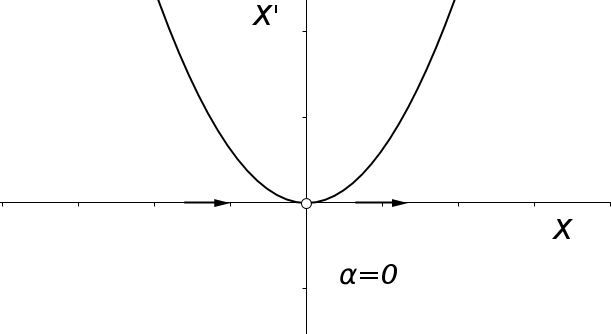
\includegraphics[width=0.5\textwidth]{saddlenode4.png}
 			\caption{Comportamiento de (\ref{sadd}) con $\alpha=0$.}
 		\end{figure}
 		\item $\alpha \in \mathbb{R^+} $ : en este caso no tenemos ningún punto fijo
 		\begin{figure}[h]
 			\centering
 			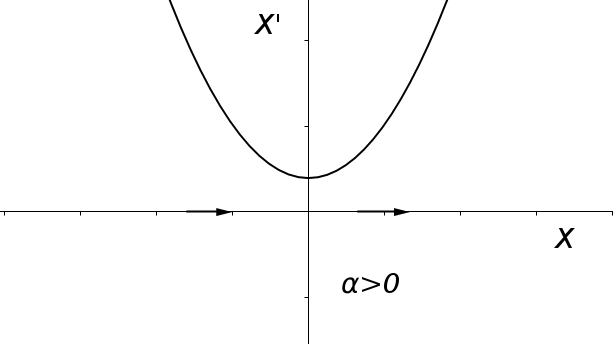
\includegraphics[width=0.5\textwidth]{saddlenode5.png}
 			\caption{Comportamiento de (\ref{sadd}) con $\alpha>0$.}
 		\end{figure}
 	\end{itemize}
 	A modo de resumen gráfico dibujaremos a continuación el diagrama de bifurcaciones de este tipo (\ref{diagfold}). Es de destacar que para comprender el gráfico basta observar que el mismo nos da información sobre la aparición y desaparición de puntos fijos y por supuesto y sobre el cambio en el diagrama de fases según $\alpha$ varía. Es por esto que $\alpha$ suele aparecer en el eje horizontal.
 	\begin{figure}[h]
 		\centering
 		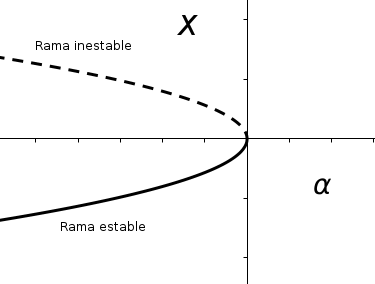
\includegraphics[width=0.5\textwidth]{saddlenodediagrama.png}
 		\caption{Diagrama de bifurcación de Saddle Node.}
 		\label{diagfold}
 	\end{figure}
 	Como veremos más adelante la bifurcación fold y la bifurcación de Hopf (que definiremos en el siguiente apartado) son de las bifurcaciones básicas más importante en biología. Esto se debe a que en el resto de bifurcaciones, bajo ligeras variaciones en los parámetros, aparecerán en nuestros diagramas zonas con un comportamiento local idéntico a la bifurcación fold. Buena prueba de ello es el tema dedicado a este fenómeno en \cite{Strogatz}. Es por eso que decidimos estudiar, a modo de ejemplo generalizable, la obtención de la forma normal de ésta.
 	
 	Para ello, basándonos en el desarrollo ejemplificado en \cite{Kuznet} o \cite{murdock}, comenzamos probando un lema sencillo que nos habla sobre la persistencia de esta bifurcación ante la introducción de nuevos términos en la expresión de $f(x,\alpha)$ lo cual nos dará vía libre para entender como tratar casos en los que aparece esta bifurcación, llegando así a su forma normal:
 	\begin{lemma}
 		Supongamos que tenemos nuestra ecuación de la forma \[ x' = {\alpha}+ x^2 .\]
 		Si añadimos a nuestra ecuación términos de orden superior\footnote{Por ejemplo: $\mathcal{O}(x^2)$ designará a expresiones  cuyo valor, cuando tiendan a infinito, quede acotado por una expresión de la forma $ax^2$, con $a$ constante } (denotados por $\mathcal{O}$) entonces el sistema de la forma:
 		\begin{equation}
 		x' = {\alpha}+ x^2 + \mathcal{O}(x^3) .
 		\label{fold3}
 		\end{equation}
 		es topológicamente equivalente en un entorno del origen a 
 		\[ x' = \alpha + x^2. \]
 		Ocurre por tanto que nuestro sistema no muestra un cambio cualitativo en su comportamiento cerca del origen.
 	\end{lemma}
\begin{proof}
	La prueba la podemos dividir en dos partes, primero analizaremos que en ambas expresiones encontramos los mismo puntos fijos (con la misma naturaleza) y luego construiremos un homeomorfismo que nos lleve de un sistema a otro. Esta prueba se fundamenta en el hecho de que para sistemas dinámicos escalares un homeomorfismo que lleve los puntos de equilibrio en puntos de equilibrio de otro sistema también hará lo propio con las órbitas.
	\begin{enumerate}
		\item Introducimos una variable escalar, de manera que nuestro sistema quede de la forma
		\[ y' = F (y, \alpha) = \alpha + y^2 + \psi(y,\alpha) .\]
		donde $ \psi = O(y^3 )$ una función de $(y,\alpha)$ continuamente diferenciable ( o $C^\infty$) en un entorno de (0, 0). Ahora, consideramos la naturaleza de la variedad que nos define el equilibrio cerca del $(0, 0)$ del plano formado por $(y,\alpha)$ :
		\[ M = \{(y,\alpha) : F (y,\alpha) = \alpha + y^2 + \psi(y,\alpha) = 0\} .\]
		En este caso podemos hablar de una curva que pasa por el origen ($F(0,0)=0$). Por el teorema de la función implícita (pues $F_\alpha(x,\alpha)=1$), admite una parametrización local como:
		\[ M = \{(y,\alpha) : \alpha = g(y)\} . \]
		con g es continuamente diferenciable y está definida para valores de $y$ cercanos a $0$. De hecho, la expresión de g nos queda
		\[ g(y) = -y^2 + \mathcal{O}(y^3) .\]
		Por tanto para pequeñas variaciones de $\alpha < 0$ tendremos comportamiento similar, es decir la existencia de dos puntos fijos cerca del origen  $y_2(\alpha), y_1(\alpha)$.
		\item Construimos ahora un homeomorfismo dependiente de $\alpha$, para valores cercanos a 0. Para valores  $\alpha \geq 0$ tomamos la aplicación identidad:
		\[ h_\alpha (x) = x .\]
		Para valores de $\alpha \textless 0$ tomamos la transformación lineal:
		\[ h_\alpha (x) = \delta (\alpha) + b(\alpha)x. \]
		donde los valores de $\delta$ y b quedan determinados por el efecto de la aplicación sobre los valores de nuestros dos puntos fijos (los de partida y los de llegada):
		\[ h_\alpha (x_j (\alpha)) = y_j(\alpha), j = 1, 2 .\]
		Tenemos por tanto un homeomorfismo $h_\alpha:\mathbb{R}^1 \to \mathbb{R}^1$, que nos lleva de unas órbitas a otras (por el resultado que señalábamos en el primer párrafo, comentado en \cite{Kuznet}), preservando la dirección del tiempo. Por tanto, por la definición de equivalencia de sistemas, tenemos el resultado.
	\end{enumerate}
\end{proof}
Este resultado nos da pie a generalizar la forma normal de la bifurcación: 
\begin{theorem}[Forma normal de la bifurcación fold]
	Supongamos el sistema 1-dimensional:
	\begin{equation}
	x'=f(x,\alpha),
	\end{equation}
	con f derivable y un punto fijo en $x=0$ cuando $a=0$. Supongamos además que verifica: $f_x(0,0)=0$, $f_{xx}(0,0) \neq 0)$ y $f_\alpha(0,0) \neq 0$ Entonces nuestro sistema tiene una bifurcación fold y su forma normal puede escribirse como: \[x'=\alpha+x^2.\]
\end{theorem}
\begin{proof}
	\textit{Skecth de la prueba}\cite{prac,Kuznet}: La idea fundamental detrás de esta demostración es, como en el lema previo, puramente constructiva. Es por ello que dejamos los pasos de la misma, aunque no profundicemos en la operaciones. 
	Dado un sistema con una función continuamente diferenciable f que posee en $\alpha=0$ un equilibrio en $x=0$ y $f_x(0,0)=0$, podemos utilizar el desarrollo en serie de Taylor para llegar a esta expresión:
	\[f(x,\alpha)=f_0(\alpha)+f_1(\alpha)x+f_2(\alpha)x^2+\mathcal{O}(x^3).  \]
	La filosofía de la prueba es, mediante cambios de variables invertibles ( y $C^\infty$) en la variable y el parámetro, transformar el sistema en uno equivalente de la forma (\ref{fold3}), y aplicar el lema demostrado.
	
	
\end{proof}


Equivalentemente podemos tratar el caso 
\begin{equation}
x'=\alpha-x^2.
\end{equation}
cuyo comportamiento es similar respecto de la variación entre $[-\infty,+\infty]$ de $\alpha$, siendo simétrico en cuanto a esquema pero permutándose las ramas estables e inestables.

Es habitual que en la clasificación de bifurcaciones no haya un consenso generalizado sobre el nombre de las mismas. Para evitar confusiones he de resaltar que esta bifurcación también recibe el nombre de bifurcación de doblez (fold bifurcation) o de punto giratorio (turning point bifurcation)


\item Bifurcación transcrita\\
Es habitual también, encontrarnos casos en los que para toda variación del parámetro encontramos existencia de puntos fijos (tanto estables como inestables). \\
Dentro de este esquema presentamos la siguiente bifurcación denominada transcrita En ella siempre, para todo valor de  $\alpha$ hallaremos la existencia  de nodos, sin embargo estos cambiarán su estabilidad.
\\
Podemos observar este comportamiento en la siguientes gráficas \ref{trans1}, \ref{trans2}, \ref{trans3}:
\begin{figure}[H]
	\centering
	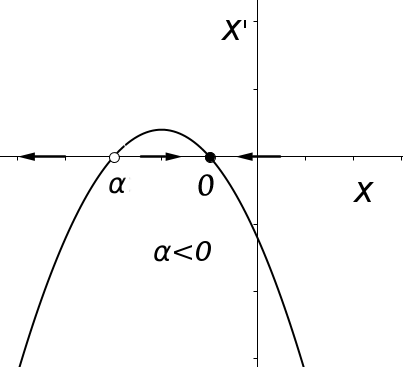
\includegraphics[width=0.45\textwidth]{trans1.png}
	\caption{Comportamiento de (\ref{trans}) en $\alpha<0$.}
	\label{trans1}
\end{figure}
\begin{figure}[H]
	\centering
	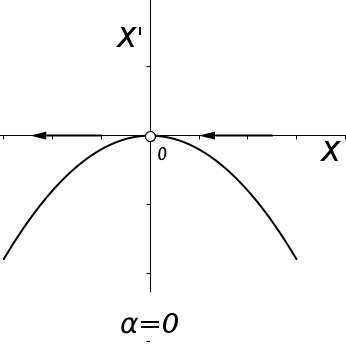
\includegraphics[width=0.45\textwidth]{trans2.png}
	\caption{Comportamiento de (\ref{trans}) en $\alpha=0$ .}
	\label{trans2}
\end{figure}
\begin{figure}[H]
	\centering
	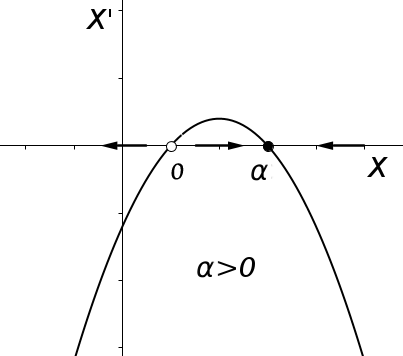
\includegraphics[width=0.45\textwidth]{trans3.png}
	\caption{Comportamiento de (\ref{trans}) en $\alpha>0$.}
	\label{trans3}
\end{figure}
Para presentar esta bifurcación recurrimos de nuevo a la forma normal:
\begin{equation}
x'=x(\alpha-x).
\label{trans}
\end{equation}
donde $\alpha$ es un parámetro que puede ser positivo, negativo o 0.
Teniendo todos los ingredientes para poder dibujar nuestro diagrama de bifurcaciones (Figura \ref{trandia}).
\begin{figure}[H]
	\centering
	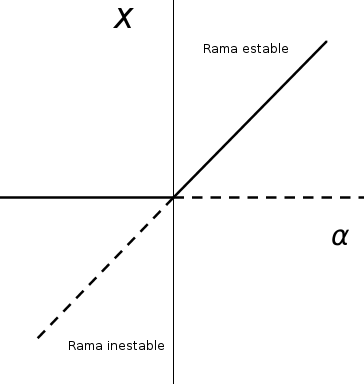
\includegraphics[width=0.5\textwidth]{trandiagrama.png}
	\caption{Diagrama de bifurcaciones de la bifurcación transcrita}
	\label{trandia}
\end{figure}

Un ejemplo trivial de este comportamiento puede verse en ecuaciones que modelizan crecimiento de poblaciones. Destacaremos su aparición en modelos epidemiológicos en los apartados de aplicaciones.


\item Bifurcación de Pitchfork

En este caso nos encontramos con una bifurcación en la cual según varía el parámetro aparecerán 3 nodos o puntos fijos (es por esto que es habitualmente llamada de tenedor o tridente). Es una bifurcación que suele aparecer en casos en los que el sistema presenta algún tipo de simetría, además también se la suele denotar biestable, debido a la aparición de las dos ramas estables cuando el parámetro crece.

Dentro de este tipo de bifurcaciones encontramos dos casos bien diferenciados:
\begin{enumerate}
	\item Bifurcación de pitchfork supercrítica
	
	La primera bifurcación de este tipo que presentamos, es la supercrítica. Recogemos aquí su forma normal de la cual comenzaremos a deducir propiedades:
	\begin{equation}
	x'=\alpha x-x^3=x(\alpha-x^2).
	\label{pitch}
	\end{equation}
	donde $\alpha$ es un parámetro que puede ser positivo, negativo o 0.
	Vemos desde un primer momento que esta función es invariante para cambios de variables del tipo: $x \rightarrow -x$. Más formalmente diremos que en este caso el campo de vectores es equivariante, es decir, que el resultado de aplicar una simetría a la función y luego representarla es lo mismo que representar la función en nuestro dominio y luego realizar la simetría.
	Vamos con la representación: \\
	\begin{figure}[H]
		\centering
		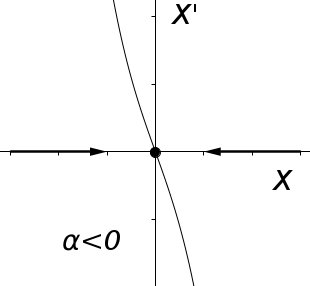
\includegraphics[width=0.45\textwidth]{pitch11.png}
		\caption{Comportamiento de (\ref{pitch}) en $\alpha<0$. }
	\end{figure}
	\begin{figure}[H]
		\centering
		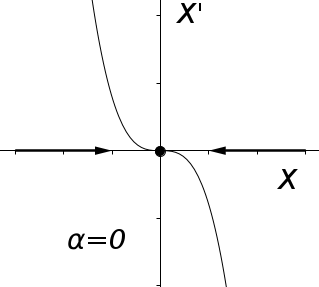
\includegraphics[width=0.45\textwidth]{picth12.png}
		\caption{Comportamiento de (\ref{pitch}) en $\alpha=0$ .}
	\end{figure}
	\begin{figure}[H]
		\centering
		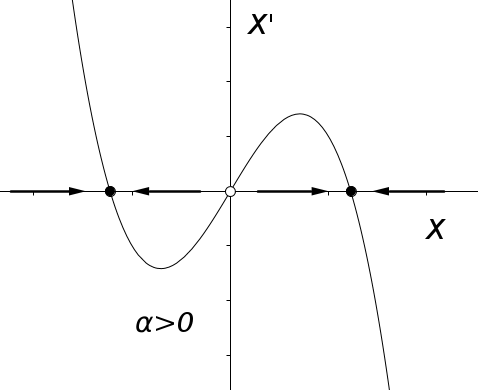
\includegraphics[width=0.45\textwidth]{picth13.png}
		\caption{Comportamiento de (\ref{pitch}) en $\alpha>0$. }
	\end{figure}
	Como podemos observar en los gráficos, cuando $\alpha$ es menor que 0 o estrictamente igual a cero siempre tenemos un punto fijo, estable en $x=0$. Sin embargo conforme nuestro parámetro tiende  cero podemos observar visualmente como \textquotedblleft la estabilidad se va haciendo cada vez más débil\textquotedblright  hasta terminar por desaparecer en 0 cuando $\alpha \textgreater 0$. Al mismo tiempo cuando esto sucede se crean dos puntos fijos estables.
	
	Una vez concluido este estudio podemos representar trivialmente el diagrama de bifurcaciones, del cual se puede comprender mejor la denotación de esta bifurcación (Figura \ref{pitch1}).\\
		\begin{figure}[H]
			\centering
			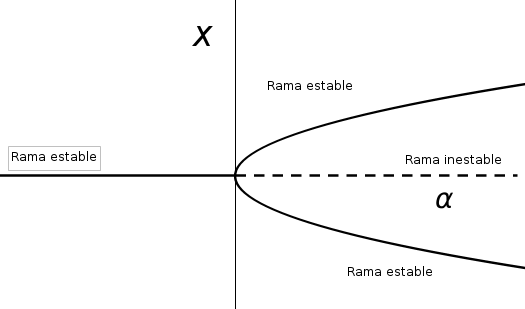
\includegraphics[width=0.5\textwidth]{pitch1diagrama.png}
			\caption{Diagrama de bifurcaciones pitchfork supercrítica.}
			\label{pitch1}
		\end{figure}
	
	\item Bifurcación de pitchfork subcrítica\\
	Discutimos ahora el siguiente caso de bifurcación tipo pitchfork: subcrítico En esta bifurcación nos encontramos ante un comportamiento de tridente gráficamente similar a nuestro anterior estudio pero en este caso predominarán los nodos inestables. Representamos a continuación el aspecto local que tienen las bifurcaciones de este tipo: 
	la forma normal de esta bifurcación es la siguiente:
	\begin{equation}
	x'=\alpha x+x^3=x(\alpha +x^2)
	\label{pitch2}
	\end{equation}
	donde $\alpha$ es un parámetro que puede ser positivo, negativo o 0.\\
	Como podemos observar la evolución de nuestro sistema según varía $\alpha$ es muy similar al caso anterior. \\Si $\alpha \textless 0$ encontraremos 2 puntos de equilibrio, dos inestables y unos estable en 0. Cuando $\alpha \geq 0$ los puntos de equilibrio confluyen en 0, quedando un solo punto fijo inestable.
	Con esta información podemos elaborar ya el diagrama de bifurcaciones \ref{pitch21}
	\begin{figure}[H]
		\centering
		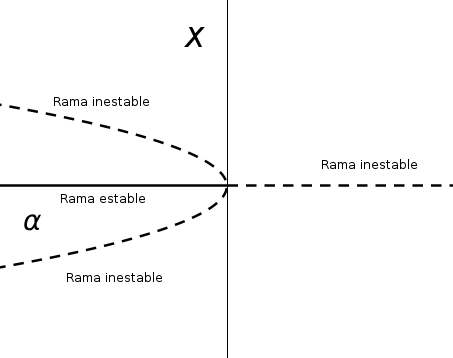
\includegraphics[width=0.5\textwidth]{pitch2diagrama.png}
		\caption{Diagrama de bifurcaciones Pitchfork subcrítica}
		\label{pitch21}
	\end{figure}
\end{enumerate}
Concluimos con esto la introducción para bifurcaciones 1-dimensionales.


 Evolucionando de estas obtendremos algunas de la bifurcaciones usuales en 2 dimensiones. Como dije al principio este estudio no es mas que una ligera pincelada de los muchos comportamientos que podemos encontrar en nuestros sistemas dinámicos.
\end{enumerate}

\subsubsection{Sistemas 2-dimensionales}
Siguiendo la filosofía del apartado inmediatamente anterior, introduciremos en este un conjunto de las bifurcaciones 2-dimensionales, que, si bien no es exhaustivo, pretende aportar una idea general, la cual, combinada con nuestros conocimientos de estabilidad de Ecuaciones Diferenciales II, nos puede dar pie a profundizar cuanto queramos. \\
Es de resaltar que en sistemas dos dimensionales nos vamos a encontrar con comportamientos similares a los que se pueden observar en una dimensión. Sin embargo en este apartado no sólo los puntos fijos se verán afectados, \textquotedblleft creándose\textquotedblright o \textquotedblleft destruyéndose\textquotedblright, sino que también lo harán las órbitas cerradas.\\
Es obvio que las bifurcaciones presentadas anteriormente tienen su análogo en 2 dimensiones, por ello, presentaremos su diagrama y su forma normal, recayendo la importancia central de este apartado en la bifurcación más representativa, no vista hasta ahora. Las gráficas mostradas en relación con las bifurcaciones saddle-node, transcrítica y fold, para mejorar su comprensión, serán los diagramas de fase con la representación de sus puntos fijos y la estabilidad de los mismos.
\begin{enumerate}
	\item Bifurcación Saddle-Node. \\
	En este como en el resto de los casos, el comportamiento a estudiar no cambia, pues está restringido a una sola dimensión. Por ello añadir más dimensiones nos muestra simplemente la forma en la que las órbitas se relacionan con este subespacio, tanto si son repelidas como atraídas.
	Dado que nuestra segunda variable no dependerá de nuestro parámetro, una vez tengamos la forma normal de la variable dependiente, para completar utilizaremos una función, que simplifique nuestros cálculos. En este caso hemos escogido una exponencial:
	\begin{equation}
	\left \{ \begin{matrix}x'=\alpha+x^2, \\y'=-y.\end{matrix}\right.
	\label{fold2d}
	\end{equation}  
	
	Encontramos por tanto el mismo comportamiento en la variable $x$ (de hecho todas las bifurcaciones de Saddle Node se comportan localmente igual), únicamente influenciado por su relación con la variable $y$ que modifica el espacio de fase.
	\begin{figure}[H]
		\centering
		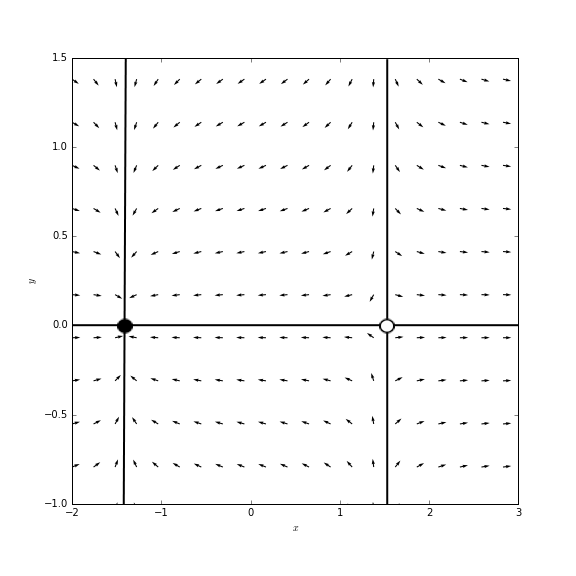
\includegraphics[width=0.45\textwidth]{fold11.png}
		\caption{Comportamiento de (\ref{fold2d}) en $\alpha<0$. }
	\end{figure}
	\begin{figure}[H]
		\centering
		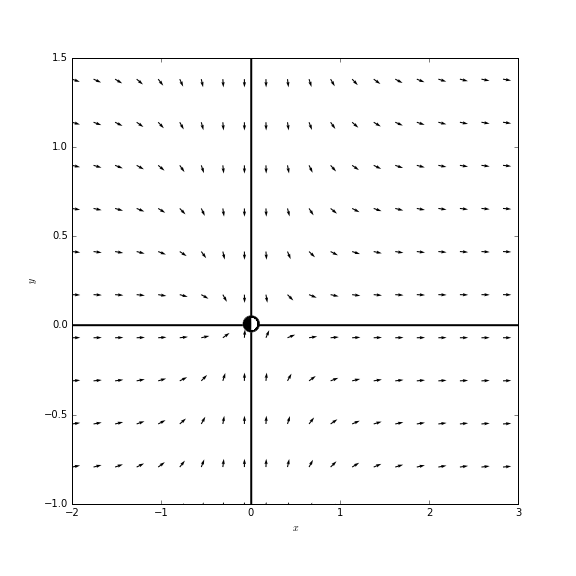
\includegraphics[width=0.45\textwidth]{fold12.png}
		\caption{Comportamiento de (\ref{fold2d}) en $\alpha=0$ .}
	\end{figure}
	\begin{figure}[H]
		\centering
		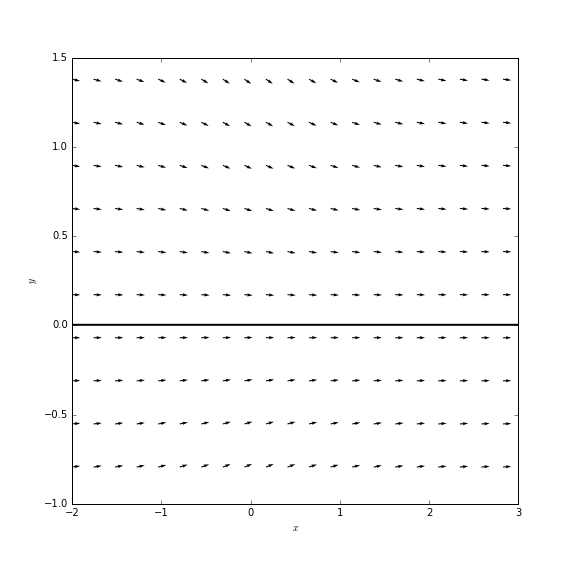
\includegraphics[width=0.45\textwidth]{fold13.png}
		\caption{Comportamiento de (\ref{fold2d}) en $\alpha>0$. }
	\end{figure}
	\item Bifurcación transcrítica. \\
	Nos encontraremos en este apartado con la forma general:
	\begin{equation}
	\left \{ \begin{matrix}x'=\alpha x-x^2 \\y'=-y\end{matrix}\right .. 
	\label{trans2d}
	\end{equation}
	Tenemos por tanto el mismo comportamiento en la variable $x$, que podemos reflejar gráficamente en los diagramas de fase. 
	\begin{figure}[H]
		\centering
		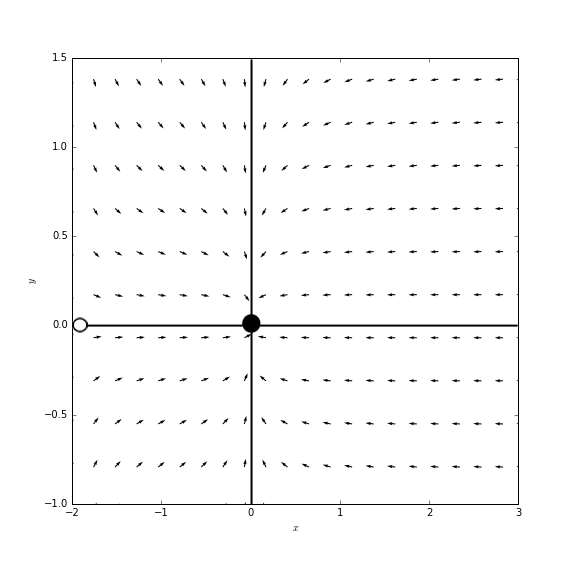
\includegraphics[width=0.45\textwidth]{trans11.png}
		\caption{Comportamiento de (\ref{trans2d}) en $\alpha<0$. }
	\end{figure}
	\begin{figure}[H]
		\centering
		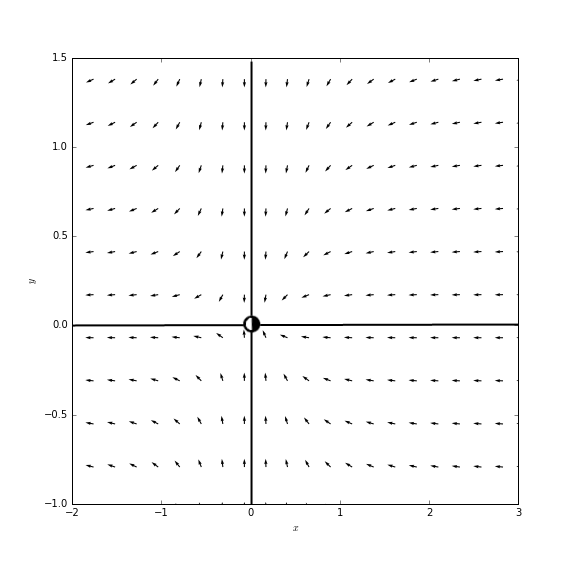
\includegraphics[width=0.45\textwidth]{trans12.png}
		\caption{Comportamiento de (\ref{trans2d}) en $\alpha=0$ .}
	\end{figure}
	\begin{figure}[H]
		\centering
		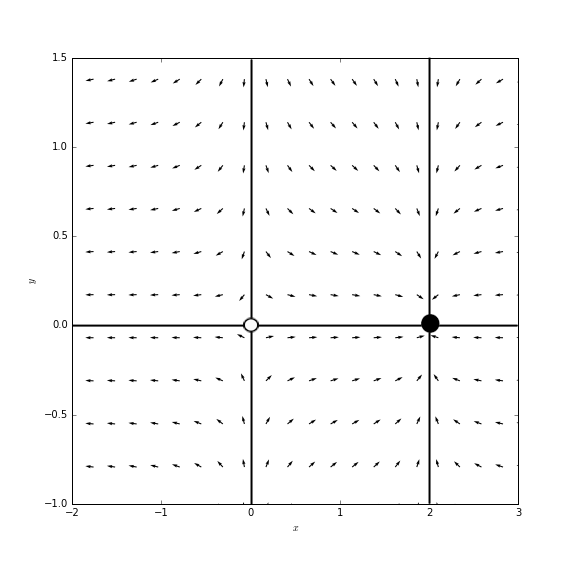
\includegraphics[width=0.45\textwidth]{trans13.png}
		\caption{Comportamiento de (\ref{trans2d}) en $\alpha>0$. } 
	\end{figure}
	\item Bifurcación Pitchfork. \\
	Juntamos en este apartado los dos tipos de bifurcación Pitchfork:
	\begin{equation}
	\left\{\begin{matrix}x'=\alpha x-x^3 \\y'=-y\end{matrix}\right..
	\label{pitch2d}
	\end{equation}
	Y la subcrítica:
	\begin{equation}
	\left\{\begin{matrix}x'=\alpha x+x^3 \\y'=-y\end{matrix}\right..
	\end{equation}
	Incluimos a modo de ejemplo, los diagramas del caso supercrítico.
	\begin{figure}[H]
		\centering
		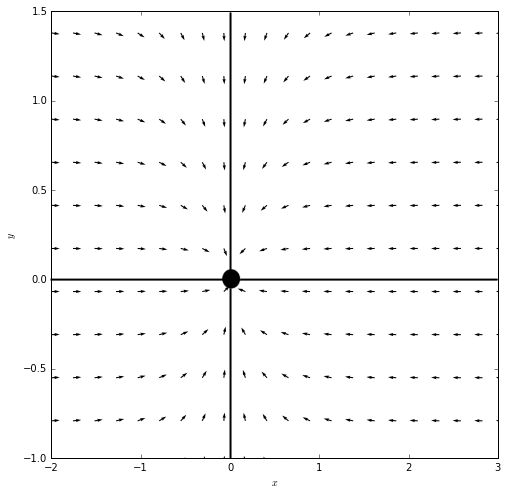
\includegraphics[width=0.45\textwidth]{pitch1.png}
		\caption{Comportamiento de (\ref{pitch2d}) en $\alpha<0$. }
	\end{figure}
	\begin{figure}[H]
		\centering
		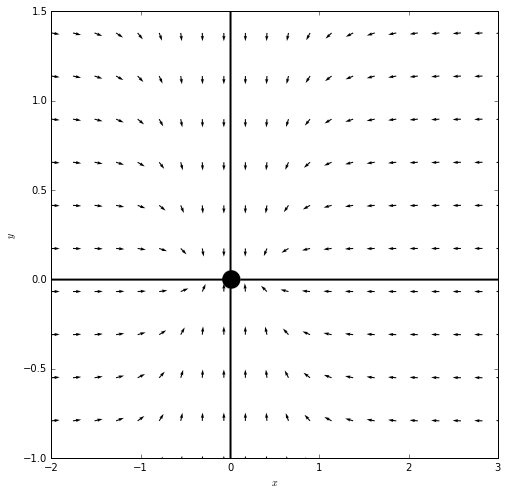
\includegraphics[width=0.45\textwidth]{pitch2.png}
		\caption{Comportamiento de (\ref{pitch2d}) en $\alpha=0$ .}
	\end{figure}
	\begin{figure}[H]
		\centering
		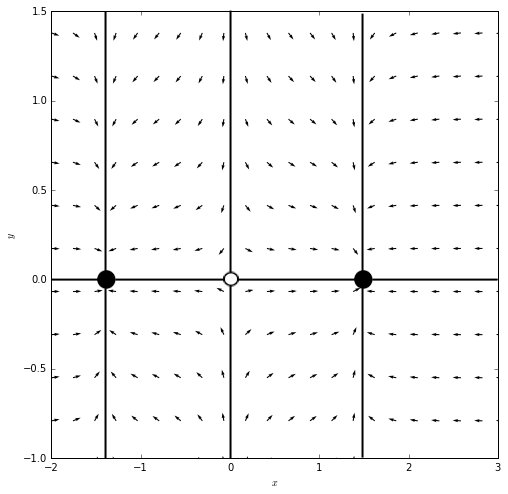
\includegraphics[width=0.45\textwidth]{pitch3.png}
		\caption{Comportamiento de (\ref{pitch2d}) en $\alpha>0$. }
	\end{figure}
	
	\item Bifurcación de Hopf o de Andronov-Hopf
	
	Hasta ahora no hemos hecho mas que extender a dos dimensiones las bifurcaciones que obteníamos en una dimensión. Esto es así por el propio carácter de los puntos fijos que estábamos considerando. Sin embargo, dado que estamos en dimensión 2, un punto fijo puede perder o modificar su estabilidad de más formas. 
	
	 Para comprender esto basta tener en cuenta como varían los valores propios del Jacobiano asociado a un sistema dinámico. Si un punto es estable los valores propios deben encontrarse en el subespacio $\Re \leq0$ (parte real menor que 0). Para que esta estabilidad cambie uno  ambos valores propios deben cruzar el eje imaginario, lo que nos ocasionará trabajar con la existencia de ciclos límite y órbitas cerradas.
	 
	Dada la importancia de esta bifurcación procederemos a estudiarla como lo hicimos con la de Saddle Node, obteniendo no solo su comportamiento sino también su forma normal. Antes de comenzar la deducción, es de destacar que al igual que en el caso de la bifurcación Pitchfork, tendremos dos tipos de bifurcación de Hopf: sub y supercrítica.\\
	Consideremos el siguiente sistema dinámico de dos variables:
	 \[ \left \{ \begin{matrix} x_1'=\alpha x_1-x_2-x_1(x_2^2+x_1^2)\\ x_2'=x_1+\alpha x_2-x_2(x_2^2+x_1^2)\end{matrix}\right.. \]
	Comprobamos que el sistema tiene puntos de equilibrio en $ x_1=0, x_2=0$:
	\begin{equation}
	\begin{split}
	&0=\alpha x_1-x_2-x_1(x_2^2+x_1^2) \\&
	0=x_1+\alpha x_2-x_2(x_2^2+x_1^2)\end{split} 
	\end{equation}
	
	
	 y, el jacobiano asociado será (tomando la parte lineal): 	 
	 \[ A= \begin{pmatrix} \alpha & -1 \\ 1 & \alpha \end{pmatrix} .\]
	cuyos valores propios serán $\lambda_{1,2} = \alpha \pm i$.
	Para estudiar el comportamiento cualitativo del sistema de forma más sencilla, dado que esto requerirá estudiar órbitas cerradas, introduciremos la variable $z$ la cual no es mas que la representación de las dos coordenadas de partida a través de un número complejo.\\
	\begin{equation}
	\begin{split}
	&z = x_1+ix_2, \\&\overline{z} = x_1-ix_2, \\ &|z|^2=z.\overline{z} = x_1^2+x_2^2.
	\end{split} 
	\end{equation}
	Esta variable satisface la ecuación diferencial,
	\[ z' = x_1' + ix_2' = \alpha(x_1 + ix_2 ) + i(x_1 + ix_2 ) - (x_1 + ix_2 )(x_1^2 + x_2^2 ). \] 
	con lo que podemos reescribir nuestro sistema inicial como: 
	\begin{equation}
	z' = (\alpha+i)z-z|z|^2 .
	\end{equation}
	Si ahora usamos el cambio de variable $z=\rho e^{i\psi}$ obtenemos, derivando:
	\[ \rho' e^{i\psi}+ i\rho\psi' e^{i\psi} = \rho e^{i\psi}(\alpha+i-\rho^2). \]
	lo cual, teniendo en cuenta el significado de la exponencial de un complejo visto en la asignatura de Variable Compleja I (fórmula de Euler), podemos traducir nuestro sistema a un sistema en coordenadas polares, el cual al estar desacoplado nos permite estudiar lo cambios cualitativos de nuestro sistema de partida según cambia el parámetro: 
	\[ \left \{ \begin{matrix} \rho' = \rho(\alpha - \rho ^2 ),\\ \psi' =1. \end{matrix}\right. \]	
	A través de esta expresión podemos deducir que $\rho$ =0 será siempre un punto de equilibrio, sin embargo su estabilidad cambiará:
	\begin{itemize}
		\item Si $ \alpha<0 $ el punto será estable (linealmente), por lo que la órbita tenderá al punto
		\item Si $\alpha=0$ el punto será estable pero no atractor, por lo que la distancia entre la solución y el punto no tiene por que disminuir exponencialmente.
		\item Si $\alpha>0$ tenemos que la estabilidad del punto cambia, para ser inestable. Sin embargo aparece una órbita cerrada, límite de todas las trayectorias en ambas componentes en $\sqrt{\alpha}$ 
	\end{itemize}
	\begin{figure}[H]
		\centering
		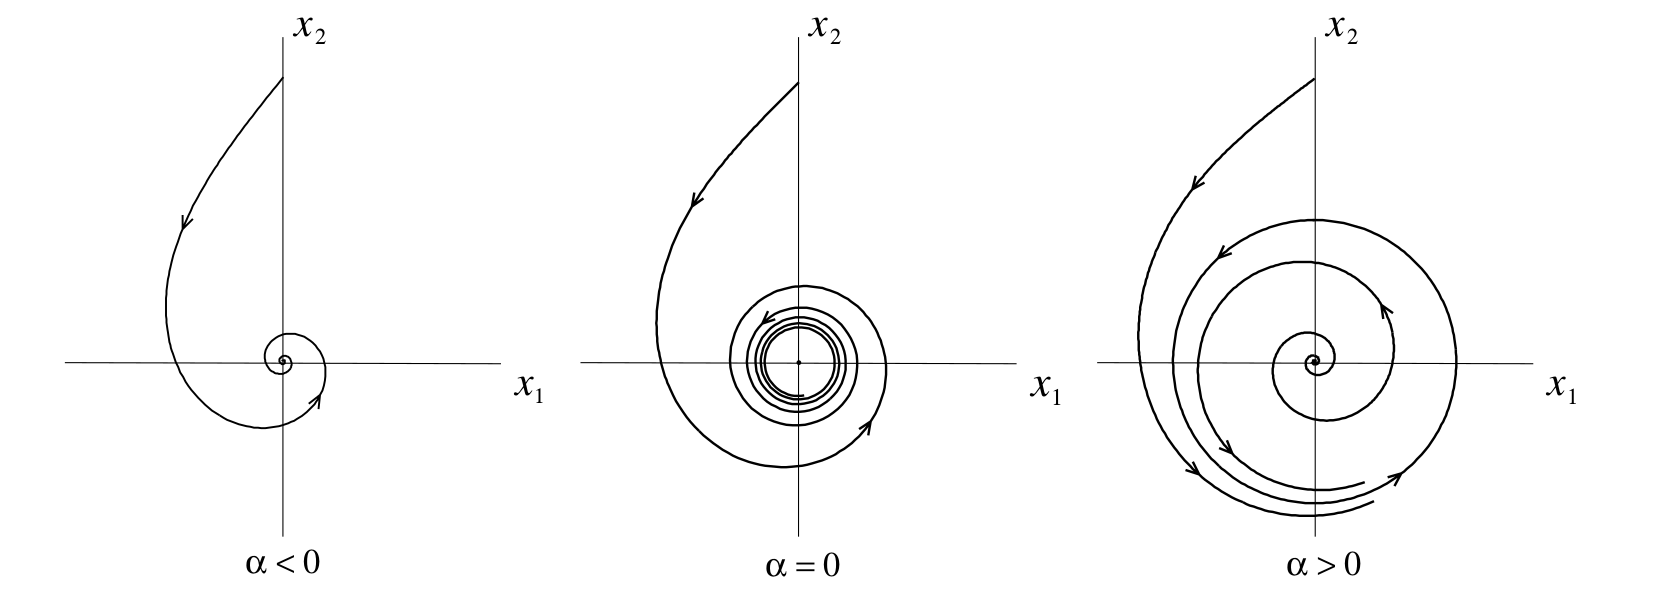
\includegraphics[width=\textwidth]{hopf11.png}
		\caption{Comportamiento Hopf supercrítica \cite{Kuznet}.}
		\label{hopf1}
	\end{figure}
	Como antes, toda esta información la podremos representar en un diagrama que nos muestre las relaciones entre x e y en varios estados de $\alpha$ o, preferiblemente, aunque quizás mas obtuso para la vista del profano, a través de un diagrama de bifurcaciones que si queremos que contenga ambas variables, será tridimensional\footnote{Veremos sin embargo, que representar tridimensionalmente diagramas de bifurcaciones suele omitirse por su costo computacional, desarrollando la mayoría de programas un gráfico que contiene toda esta información pero representable en 2 dimensiones}.
	
	Acabamos de describir la bifurcación de Hopf Supercrítica. Como avanzábamos, existe también la Hopf subcrítica:\[ \left \{ \begin{matrix} x'=\alpha x-y+x(y^2+x^2)\\ y'=x+\alpha y+y(y^2+x^2)\end{matrix}\right . .\]
	la cual, tras un cambio análogo, puede ser descrita como sigue:\[ \left \{\begin{matrix} \rho' = \rho(\alpha + \rho ^2 ),\\ \psi' =1 \end{matrix}\right .. \]
	Evidentemente encontramos un cambio notable en el comportamiento de las soluciones:
	\begin{itemize}
		\item Si $\alpha<0$ el punto 0 será un punto de equilibro estable, pero encontraremos una órbita límite inestable de radio $\sqrt{|\alpha|}$
		\item Si $\alpha=0$ La órbita límite desaparece, aunque el origen conserva la estabilidad.  
		\item Si $\alpha>0$ el punto será inestable, y con una velocidad de repulsión exponencial.
	\end{itemize}
		\begin{figure}[H]
			\centering
			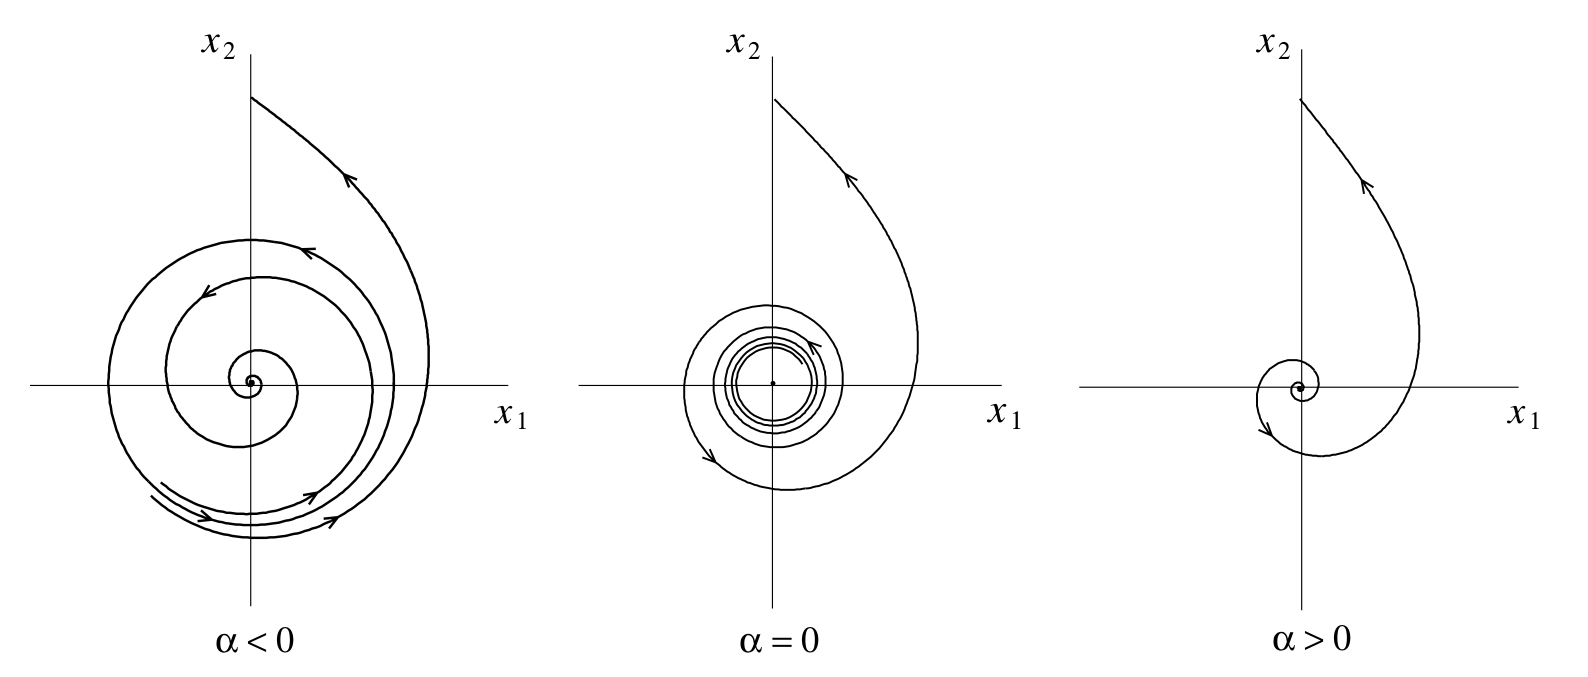
\includegraphics[width=\textwidth]{hopf21.png}
			\caption{Comportamiento Hopf subcrítica \cite{Kuznet}. }
		\label{hopf2}
	\end{figure}
	
	Presentamos de nuevo, para aclaración los diagramas de bifurcaciones. En este caso serán más difíciles de visualizar puesto que al tener un sistema 2-dimensional, la representación completa del diagrama es 3-dimensional.

\begin{figure}[H]
	\centering
	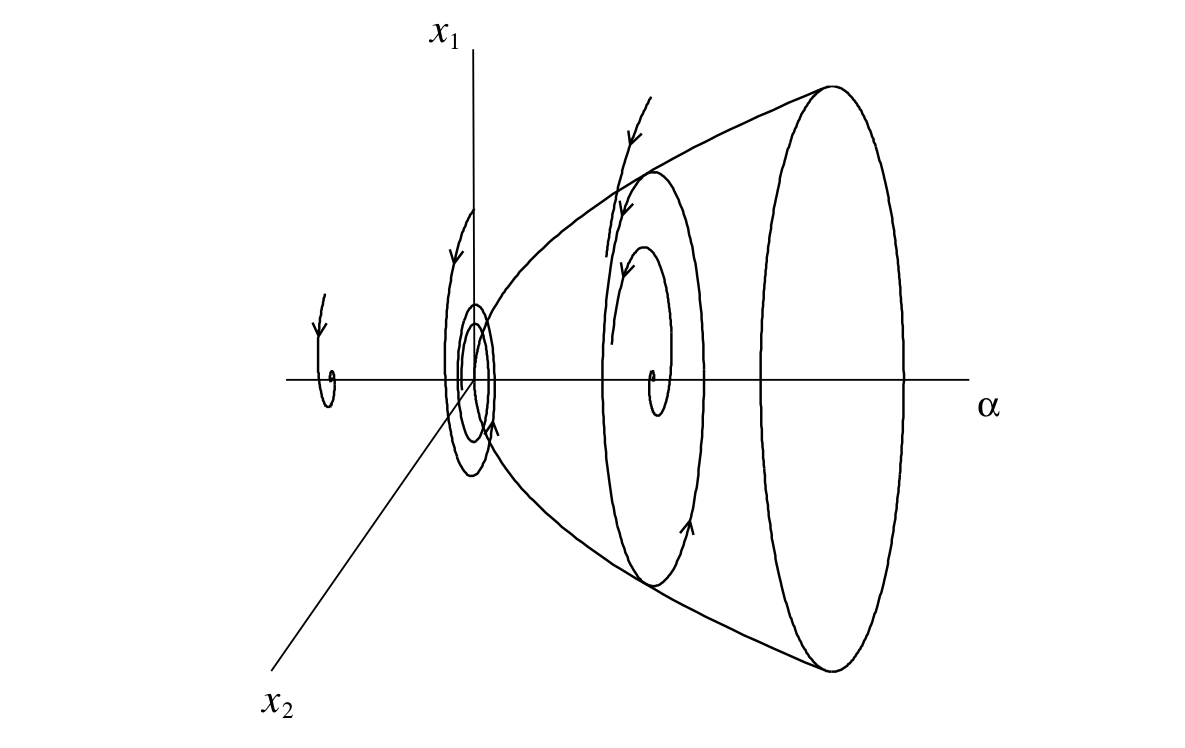
\includegraphics[width=\textwidth]{hopf12.png}
	\caption{Diagrama de bifurcaciones Hopf supercrítica\cite{Kuznet}. }
\label{hopf3}
\end{figure}
\begin{figure}[H]
	\centering
	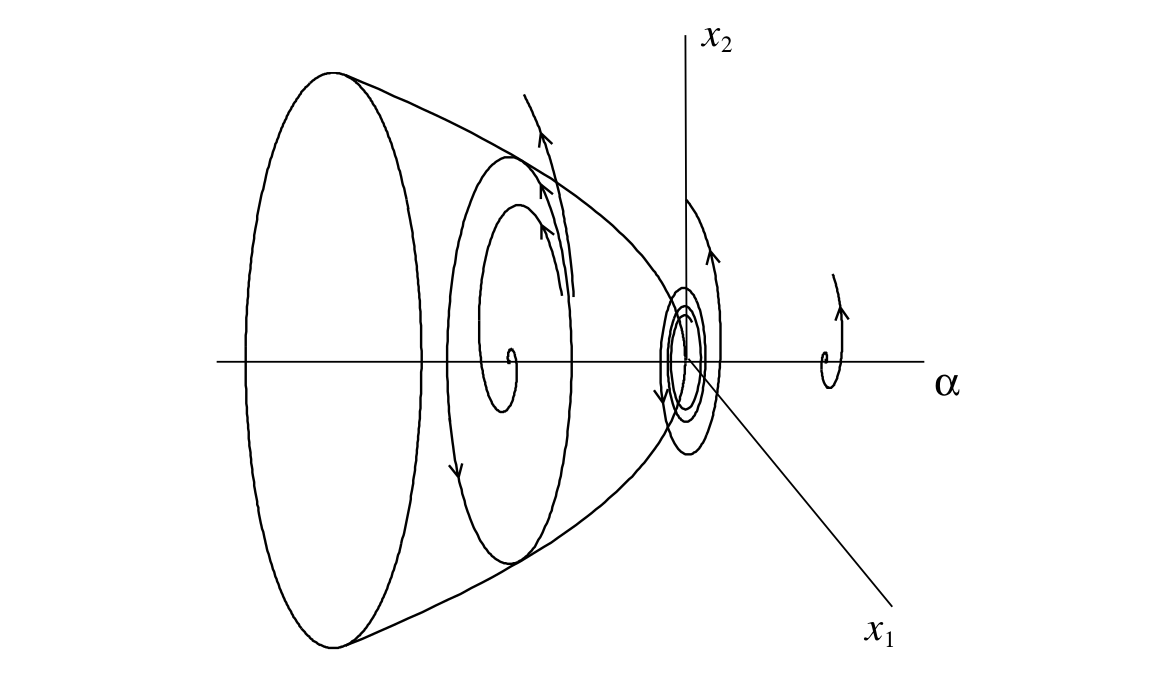
\includegraphics[width=\textwidth]{hopf22.png}
	\caption{Diagrama de bifurcaciones Hopf subcrítica \cite{Kuznet}. }
\label{hopf4}
\end{figure}
	Finalmente incluimos un resultado sobre la forma normal de la bifurcación. Si bien el resultado no nos permite estrictamente conocer la forma normal de esta bifurcación, nos ayuda a dar el primer paso en este sentido. Con el podemos concluir como términos de mayor orden no afectan localmente a nuestra bifurcación, con lo que podremos usar el término de localmente topológicamente equivalentes. Este resultado sirve como catalizador para probar que cualquier sistema, verificándose las hipótesis adecuadas, en el que haya una bifurcación de Hopf, puede ser escrito localmente a través de la forma normal que damos a continuación, concluyendo así el resultado.
	\begin{lemma}
		El sistema 
		\begin{equation}
		\begin{pmatrix}
		x_1' \\
		x_2'
		\end{pmatrix}
		=
		\begin{pmatrix}
		\alpha & -1\\
		1 & \alpha
		\end{pmatrix}
		.
		\begin{pmatrix}
		x_1 \\
		x_2
		\end{pmatrix}
		-(x_1^2+x_2^2)
		\begin{pmatrix}
		x_1 \\
		x_2
		\end{pmatrix}
		+O(x^4).
		\end{equation}
		es localmente topológicamente equivalente cerca del origen a \[ \left \{ \begin{matrix} x'=\alpha x-y-x(y^2+x^2)\\ y'=x+\alpha y-y(y^2+x^2)\end{matrix}\right . .\]
	\end{lemma}
	
	La prueba aunque extensa\footnote{Puede consultarse en el capítulo 3 de \cite{Kuznet}.}, sigue la misma filosofía que la realizada para bifurcación de fold, con ligeras variaciones (como el estudio de la existencia del ciclo límite), dejándonos la forma normal que hemos presentado al principio del apartado.
	
	Esta caracterización responde a un estudio más analítico que cualitativo. Sabemos que la bifurcacion de Hopf se comportarán de una forma similar al comportamiento observado en la forma normal, esto es, los resultados analíticos que apliquemos a la forma normal serán extensibles a nuestro sistema. \\
	
	
	Acabamos, por tanto, exponiendo una caracterización que supondrá un criterio a evaluar cuando necesitemos saber si nos encontramos ante una bifurcación de Hopf. 
	De nuevo la motivación de algunas hipótesis nace en la construcción de la forma normal (genérica) al igual que acontecía en la bifurcación fold.
	
	\begin{theorem}
		Consideremos el sistema:
		\[ \left \{ \begin{matrix} x'=f(x,y,\alpha)\\ y'=g(x,y,\alpha)\end{matrix}\right . .\]
		Donde $alpha$ es nuestro parámetro. Supongamos que tenemos un punto fijo $(x,y)=(x_0,y_0)$ y supongamos que los valores propios del sistema linealizado en un entorno del punto son: $\lambda_{1,2}=a(\alpha)\pm ib(\alpha)$.
		
		Supongamos ahora que para un valor de $\alpha=\alpha_0$ se verifican:
		\begin{enumerate}
			\item $a(\alpha)=0$, $b(\alpha)=\omega\neq0$ donde $sgn(\omega)=sgn[(g_x(x_0,y_0,\alpha_0))]$\\(esta condición nace de la exigencia de tener un par de valores propios imaginarios)
			\item $a_\alpha(\alpha_0)\neq0$\\(Esta condición se obtiene al imponer el cruce del eje imaginario por parte de estos valores)
			\item $\delta=\frac{1}{16}(f_{xxx}+f_{xyy}+g_{xxy}+g_{yyy})+\frac{1}{16\omega}(f_{xy}(f_{xx}+f_{yy})-g_{xy}(g_{xx}+g_{yy})-f_{xx}g_{xx}+f_{yy}g_{yy})$\\(esta condición se obtiene durante la demostración, para justificar que los cambios de variable que se efectúan en ella pueden hacerse)
		\end{enumerate}
		\label{teoremahopf}
	\end{theorem}
	La prueba completa del teorema puede consultarse en \cite{andronof} donde está demostrada por Andronov en su versión en dimensión dos. Si se quiere una generalización se puede consultar\cite{hopfbif} para la traducción de la demostración de Hopf de la extensión de este resultado a dimensión n.
	
\end{enumerate}

\section{Revisitando los osciladores}
Como primera aplicación de este apartado, vamos a recuperar el ejemplo de los osciladores. Comprobamos anteriormente la existencia de órbitas cerradas y ciclos límite. Estudiando este problema sería natural preguntarse si nos encontramos ante una posible bifurcación de Hopf si dejamos libre algún parámetro.
Consideremos de nuevo\ref{vanderpol}:
\begin{equation}
x''-\alpha(1-x^2)x'+x=0.
\end{equation}
Reescribamos el sistema como uno de dos dimensiones de la forma:
\begin{equation}
\left \{ \begin{matrix} x'=y\\ y'=-x+\alpha(1-x^2)y\end{matrix}\right . .
\end{equation} 
Ya sabemos que el único punto de equilibrio es el origen. La matriz Jacobiana del sistema linealizado en un entorno del mismo será:
\begin{equation}
\begin{pmatrix}
0&1 \\
-1 & \alpha
\end{pmatrix}
\label{valooor}
\end{equation}
Por lo que los valores propios de \ref{valooor} serán:\[\lambda_{1,2}=a(\alpha)\pm b(\alpha)=\frac{\alpha\pm i\sqrt{4-\alpha^2}}{2} \]
Comprobamos ahora que se cumplen las hipótesis de \ref{teoremahopf}:
$a(0)=0$, $\omega=b(0)=-1\neq 0$, $a_\alpha(0)=0.5\neq0$.
Por último basta comprobar que $\delta=-1/8\neq 0.$

Estamos pues ante la existencia de una bifurcación de Hopf si variamos el parámetro que aparece en nuestro sistema.Dejamos además un par de gráficas en las que se puede observar este comportamiento: \ref{vander1} y \ref{vander2}

 \begin{figure}[H]
 	\centering
 	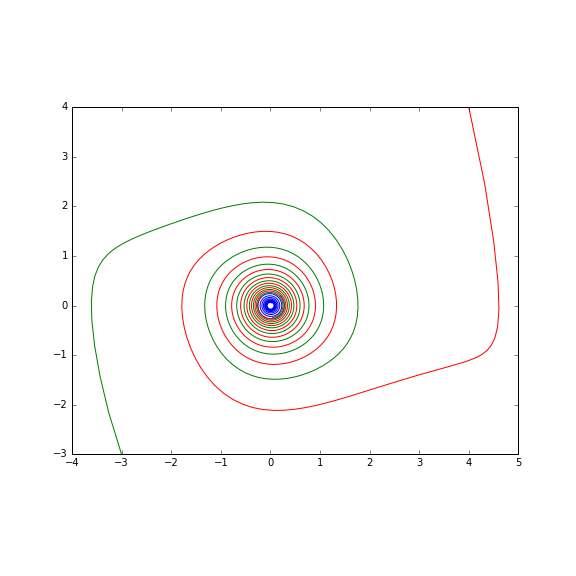
\includegraphics[width=0.5\textwidth]{vanderpol_oscillator2.png}
 	\caption{Comportamiento del oscilador de van der pol con $\alpha=-0.2$}
 	\label{vander1}
 \end{figure}

 \begin{figure}[H]
 	\centering
 	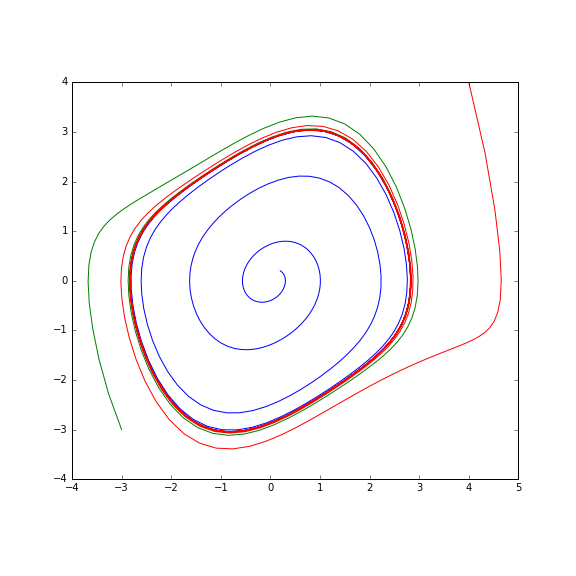
\includegraphics[width=0.5\textwidth]{vanderpol_oscillator.png}
 	\caption{Comportamiento del oscilador de Van der Pol con $\alpha=2.0$ }
 	\label{vander2}
 \end{figure}


\section{Población de gusanos de las píceas}
Uno de los primeros ejemplos de aplicación de estos conceptos se puede encontrar en el estudio de la población de los gusanos de las píceas. El modelo es sencillo, pero lo usamos por que hace aflorar como hasta los esquemas más simples de bifurcación se pueden usar en casos reales.\\
Los gusanos de las píceas son un grupo de insectos con características muy similares dentro del género \textit{Choristoneura}. La mayoría conforman plagas serias para la población de coníferas. Hay cerca de cuarenta especies de Choristoneura, e incluso más subespecies, o formas, con una gran variación entre poblaciones encontradas a través de Estados Unidos y Canadá, y en Eurasia. \\
En particular, como se señala en \cite{Strogatz}, estas plagas ocasionan graves daños al este de Canadá pudiendo acabar con grandes poblaciones de coníferas durante 4 años. 
Es por esto que surgió la necesidad de comprender la dinámica de esta población para predecir cuando encontraríamos explosiones demográficas.
Destacamos que en este modelo no influye la población de árboles, pues su crecimiento es tan lento, que a efectos prácticos su número se considera como una constante \cite{ludw}.

El modelo poblacional responde a la expresión:
\[ y'=Ry\left( 1-\frac{y}{K}\right) -p(y). \]
Donde $y(t)$ representa el número de gusanos de la población, $R$ la tasa de crecimiento y $K$ la capacidad de carga del ecosistema. En ausencia del término $p(y)$ tendríamos un modelo logístico habitual. $P(y)$ es añadido como una tasa que representa la perdida de individuos de la población debido a causas externas (generalmente predadores). Aunque se puede prestar a confusión el porqué esta tasa depende del número de gusanos, tiene una explicación biológica sencilla: cuando el número de gusanos es pequeño los depredadores ignoran las presas (pues cuesta más encontrarse con una de ellas o cazarlas en particular), sin embargo, cuando el número es muy alto, los depredadores aprovechan para alimentarse lo máximo posible. \\
Vamos a profundizar en el caso tratado por Ludwig en 1978 \cite{ludw}, siguiendo el esquema de \cite{Strogatz} a partir de la definición de $p(y)$: 
\[p(y)=\frac{By^2}{A^2+y^2},\]
con las constantes $A$, $ B$ positivas. Quedando nuestro sistema como:
\begin{equation}
y'=Ry\left( 1-\frac{y}{K}\right) -\frac{By^2}{A^2+y^2}.
\label{gusanosss}
\end{equation} 
Para trabajar con (\ref{gusanosss}) vamos a adimensionalizar el sistema. Para ello comenzamos dividiendo por $B$ y haciendo el cambio de variable $y=x/A$,lo que nos deja:
\begin{equation}
\frac{A}{B}\frac{dx}{dt}=\frac{R}{B}x\left( 1-\frac{Ax}{K}\right) -\frac{x^2}{1+x^2}.
\label{gusanossss}
\end{equation} 
Usando esta expresión podemos adimensionalizar el sistema. Para ello llamemos:
\begin{itemize}
	\item $\tau=Bt/A,$
	\item $r=RA/B,$
	\item $k=K/A.$
\end{itemize}
Entonces nuestra ecuación (\ref{gusanossss}) así adimensionalizada queda:
\begin{equation}
\frac{dx}{d\tau}=rx(1-x/k)-\frac{x^2}{1+x^2}.
\label{gusaca}
\end{equation}

Analicemos ahora la estabilidad del sistema:
comencemos por los puntos fijos, que vendrán dados por la ecuación:
\begin{equation}
\begin{split}
0=\frac{dx}{d\tau}=rx(1-x/k)-\frac{x^2}{1+x^2}\Leftrightarrow \\\Leftrightarrow \left \{ \begin{matrix} r(1-\frac{x}{k})=\frac{x}{1+x^2},\\ x=0.\end{matrix}\right .  \label{gusaco}
\end{split}
\end{equation}
Tenemos en primer lugar como punto fijo al $0$, el cual es siempre inestable, algo que podemos comprobar estudiando el signo de la derivada en un entorno del punto cuando $x$ es positivo (no tendría sentido que fuera menor que cero):
\[\text{Sea  }  0<x<k \Rightarrow rx-rx^2/k-\frac{x^2}{x+x^2}>0.\]

Esto se debe a que en un entorno de cero, el término lineal prevalece sobre los cuadráticos. Además, de la igualdad (\ref{gusaco}) podemos ver que para obtener el resto de puntos fijos, basta representar ambas funciones.
Fijado $r$ si variamos $k$ tendremos al menos un punto de intersección, hasta un máximo de 3, en los cuales la función que define nuestro sistema irá alternando estabilidad. Gráficamente podemos observar este comportamiento cualitativo de forma sencilla (Figura \ref{gusanos}).
 \begin{figure}[H]
 	\centering
 	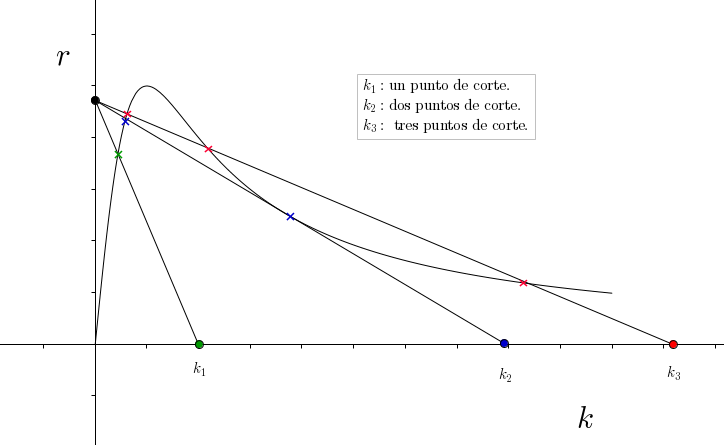
\includegraphics[width=0.8\textwidth]{gusanos.png}
 	\caption{Comportamiento de los puntos fijos según el desplazamiento de k.}
 \label{gusanos}
\end{figure}
Conforme la recta $r,k$ entre en contacto con la curva fijada por x en la segunda parte de la igualdad de (\ref{gusaco}) tendremos la aparición de dos nuevos puntos fijos. Este esquema coincide con el de una bifurcación de fold. 

¿Qué conclusiones podemos obtener?
Debido al cambio de la estabilidad de los puntos fijos, fijado $r$ podemos decir que según aumentemos $k$ tendremos dos regiones de estabilidad determinadas por los dos puntos estables que aparecen. El punto inestable que se origina cuando las nulclinas se intersecan podría entenderse como una cota de cuando el número de insectos va a crecer de forma rápida hasta alcanzar una nueva cantidad de población mayor (Figura \ref{gusanos2}).
 \begin{figure}[h]
 	\centering
 	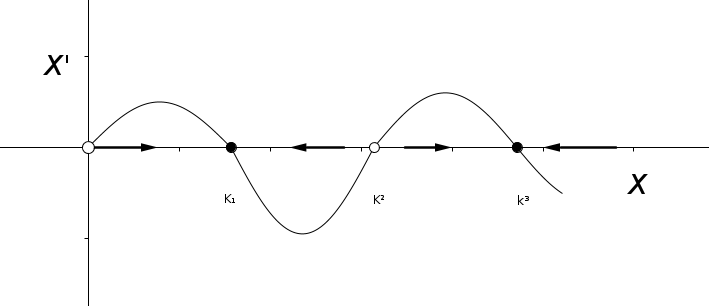
\includegraphics[width=0.5\textwidth]{gusanos2.png}
 	\caption{Estabilidad de los puntos en el caso de mayor k }
 \label{gusanos2}
\end{figure}
Este modelo podría utilizarse para estudiar cuándo las plagas de insectos van a experimentar una explosión demográfica y ajustar el término de sustracción de individuos para que esto no ocurra. 
\section{Glicólisis celular}
Como avanzábamos la bifurcación de Hopf es una bifurcación aplicable a varios campos de la biología, desde poblaciones a dinámica celular.\\En este apartado tratamos un proceso bioquímico fundamental dentro de la biología de la célula. Hablamos de la glicólisis. Mediante este proceso las células vivas obtienen energía metabolizando el azúcar. En células como la levadura, o células musculares, la glicólisis exhibe un comportamiento oscilatorio con las concentraciones de los productos intermedios creciendo y decreciendo en ciclos.

El modelo fue propuesto por Sel'kov en 1986 \cite{sel}. Las variables del mismo representan las concentraciones de ADP (adenosín difosfato) y F6P (fructosa-6-fosfato), además el modelo habitual es completado con dos parámetros que se suponen positivos.\\
El estudio expuesto está basado en los modelos estudiados en \cite{gold} y en \cite{Strogatz}. Desarrollaremos algunas de las operaciones que se realizan para estudiar el modelo, detallando los pasos analíticos a seguir. 

Partimos del sistema adimensionalizado, donde $a$ y $b$ son parámetros positivos \cite{sel}:
\begin{equation}
 \left \{ \begin{matrix} x'=-x+ay+x^2y=f(x,y)\\ y'=b-ay-x^2y=g(x,y).\end{matrix}\right .
\end{equation}
Comencemos el estudio cualitativo del sistema aplicando los conocimientos de la teoría de Poincaré Bendixson, pues observamos en los diagramas de fases la presencia de lo que podría ser comportamiento periódico (Figura \ref{hopf9}).
\begin{figure}[h]
	\centering
	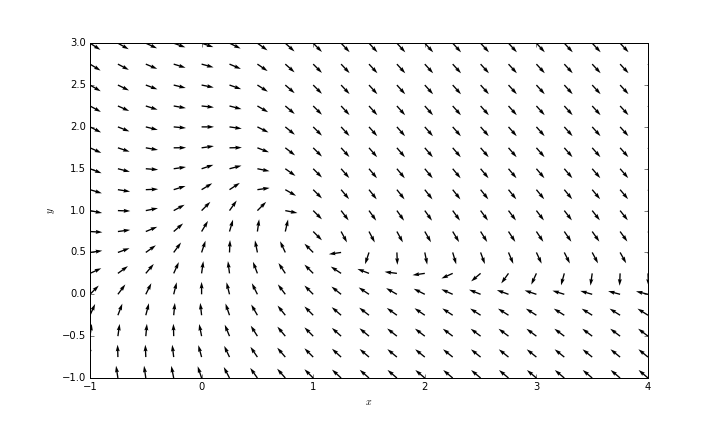
\includegraphics[width=0.7\textwidth]{selkovvv.png}
	\caption{Diagrama de fases de Sel'kov para a=0.5 y b=1 }
	\label{hopf9}
\end{figure}
Dispongamos de las nulclinas del sistema, y además dibujemos los vectores representativos según la zona del espacio en la que nos encontremos. Para ello basta conocer que la dirección del flujo viene determinada por los signos de los vectores. 

\begin{figure}[H]
	\centering
	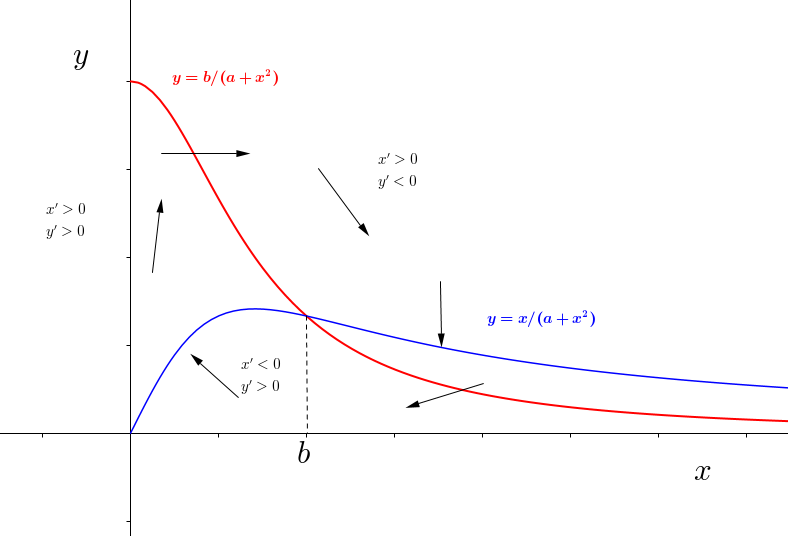
\includegraphics[width=1\textwidth]{hopfnulclinas.png}
	\caption{Nulclinas del modelo de Sel'kov }
\label{hopf7}
\end{figure}

Consideremos una región que atrape las órbitas circulares pues, al respresentar el diagrama de fases, intuimos que esta puede existir. Por ello estudiamos cómo, la región bordeada en la figura \ref{hopf8} es una región dinámicamente invariante, es decir, que cualquier órbita entrante permanecerá en ella.\\ Una posible elección de la frontera podría ser ésta:
\begin{itemize}
	\item $c_1:\left\lbrace x=0;\text{ } 0\leq y\leq b/a\right\rbrace. $
	\item $c_2:\left\lbrace 0\leq x\leq b;\text{ } y= b/a\right\rbrace. $
	\item $c_3:\text{recta entre }(b,b/a)\text{ y la nulclina de x}. $
	\item $c_5:\left\lbrace x=3b;\text{ } 0\leq y\leq \text{punto de corte con la nulclina:}\frac{3b}{a+9b^2}\right\rbrace. $
	\item $c_5:\left\lbrace y=0;\text{ } 0\leq x\leq 3b\right\rbrace. $
	
\end{itemize}
En ella podemos estudiar el comportamiento de los vectores dirección dados por el sistema: 

\begin{figure}[H]
	\centering
	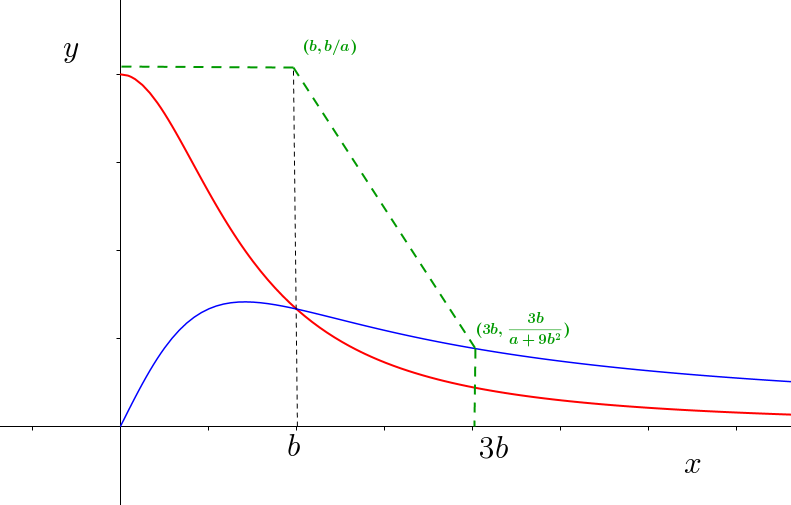
\includegraphics[width=0.7\textwidth]{areahopf.png}
	\caption{Área donde que encierra las órbitas del modelo }
\label{hopf8}
\end{figure}
\begin{itemize}
	\item Para rectas verticales y horizontales, es decir para $ x=0$ $y=0$ no hay problema, el estudio anterior nos confirma el resultado, ya que $f(0,y)=ay\geq0$ y $g(x,0)=b>0$.
	\item La recta que completa nuestra región, es la que va desde el punto $(b,b/a)$ hasta la intersección con la nulclina de $x$. Si tenemos en cuenta que para valores grandes $y'/x'$ se aproxima a  $-1$ esto nos sugiere que para acabar nuestro razonamiento debemos comparar los tamaños de $x'$ e $y'$ para valores suficientemente grandes. Consideramos $x'-(-y')$ y deducimos
	\begin{equation}
	x'-(-y')=-x+ay+x^2y+(b-ay-x^2y)=b-x
	\label{hopf5}
	\end{equation} 
	Por (\ref{hopf5}) tenemos que $-y>x'$ si $x>b$ esto implica que el vector al tener una pendiente más negativa que la recta apuntará hacia el interior de la región que hemos definido.
\end{itemize}
Tenemos pues una región cerrada y acotada, además sabemos que, si existe un valor para $b$ de manera que el punto fijo que aparece en el sistema es de naturaleza inestable, entonces, usando el teorema de Poincaré Bendixson, obtendremos la existencia de ciclos límite.

¿Ahora bien, cómo cambia nuestro sistema una vez fijado $a$?

Para ello deberemos estudiar cómo cambia la estabilidad del punto de corte. Comenzamos calculando el jacobiano:
\begin{itemize}
	\item $\partial f/\partial x=-1+2xy .$
	\item $\partial f/\partial y=a+x^2 .$
	\item $\partial g/\partial x=-2xy. $
	\item $\partial g/\partial y=-(a+x^2). $
\end{itemize}
Por lo que:
\begin{equation}
 J=\left( \begin{array}{ccc}
-1+2xy & a+x^2 \\
-2xy & -(a+x^2) \end{array} \right).
\end{equation}

Además equilibrio del sistema está en :
\[\left\lbrace  \begin{array}{ccc}
-x+ay+x^2y=0,  \\
b-ay-x^2y=0\Rightarrow -b+ay+x^2y=0.
\end{array} \right.
\]
Desde ahi, es claro que para que ambas ecuaciones se anulen, $x=b$ y con esto, sólo queda despejar $y$ de cualquiera de las dos:
\[\begin{pmatrix}
x^*=b \\
y^*=\frac{b}{a+b^2}
\end{pmatrix}.
\]
desde aquí es sencillo estudiar el determinante y la traza de jacobiano en ese punto:
\[\left\lbrace  \begin{array}{ccc}
det(J)=a+b^2>0,  \\
Traza(J)=-\frac{b^4+(2a-1)b^2+(a+a^2)}{a+b^2}.
\end{array} \right.
\]
Si $Traza(J)>0$ no encontraremos con un punto inestable por tanto habrá un ciclo límite. Si $Traza(J)<0$ tendremos uno estable y estaremos ante una espiral.\\
Este es el comportamiento básico de una bifurcación de Hopf pero esto es una mera observación, tenemos que utilizar nuestro criterio. Sin embargo, no debemos olvidar que, tras las cuentas, para comprobar la caracterización ofrecida, deberemos fijar un parámetro (en la formulación de nuestro problema aparecen 2).
 \\
Para ello, con vistas a que el valor del punto fijo interfiera lo menos posible en nuestros cáculos, vamos a desplazarlo al punto $(0,0)$ ,hallando un sistema equivalente. No sólo es una elección que facilita las cuentas, esta decisión también, en el hipotético caso en el que quisiéramos seguir trabajando en nuestro modelo, nos permitiría usar la forma normal para estudiar el comportamiento o las propiedades en las que estemos interesados en un entorno del punto fijo a través de la más sencilla forma normal.
Recogemos aquí los cálculos principales para este propósito:

Si desplazamos el punto hasta $(0,0)$ a través de una sencillo cambio de variables:$\hat{x}=x-b$ y $\hat{y}=y-\frac{b}{a+b^2}$, las derivadas de ambas coinciden y podemos expresar el sistema de la siguiente forma:
\[ \left \{ \begin{matrix} x'=-(x+b)+a(y+\frac{b}{a+b^2})+(x+b)^2(y+\frac{b}{a+b^2}),\\ y'=b-a(y+\frac{b}{a+b^2})-(x+b)^2(y+\frac{b}{a+b^2}). \end{matrix}\right . \]
donde el punto de equilibrio ya está en $(0,0)$.
Calculamos ahora los valores propios de su matriz jacobiana:
\[\begin{pmatrix}
-1+\frac{2b^2}{a+b^2} & a+b^2 \\\frac{-2b^2}{a+b^2} & -a-b^2
\end{pmatrix}.
\]
 de donde los valores propios obtenidos serán:

\[ \lambda_{1,2}(a,b)=\frac{a+a^2-b^2+2ab+b^4\pm i \sqrt{4(a+b^2)^3-(a(1+a)+(-1+2a)b^2+b^4)^2}}{-2(a+b^2)}.\]
Al final del procedimiento vamos a fijar el parámetro $a$, por lo que a la hora de comprobar si se satisfacen las condiciones será el valor de $b$ el utilizado (por lo que durante los cálculos dependerá de $a$).

Para que la parte real se anule necesitamos:
\[ b_{1,2}=\sqrt{(1\pm\sqrt{1-8a}-2a)/2} .\]
La segunda condición (que recordemos exige derivar respecto de un parámetro y nosotros hemos elegido $b$) impone:

Si $b=b_1(a)$:
\[ \frac{d\Re(\lambda_1)}{db}=\frac{\sqrt{2-16a}\sqrt{(1-\sqrt{1-8a}-2a)}}{(1-\sqrt{1-8a})}. \]
Si $b=b_2(a)$:
\[\frac{d\Re(\lambda_2)}{db}=\frac{\sqrt{2-16a}\sqrt{(1+\sqrt{1-8a}-2a)}}{(-1-\sqrt{1-8a})}.\]

Por último el valor de la expresión de la tercera condición para $b_1$ y $b_2$ vendrá determinado por:
\[-\frac{1}{8}-\frac{(a+b^2)(\frac{b}{a+b^2}+y)^3}{2\sqrt{4(a+b^2)^3-(a(1+a)+(-1+2a)b^2+b^4)^2}}\]

Por tanto, fijado $a$, podremos conocer el valor de $b$ sea nuestra elección cualquiera de las dos posibles y determinar si se cumplen las condiciones de la caracterización. En los $b$ en los que esto ocurra podremos afirmar tener una bifurcación de hopf y, dado que hemos desplazado nuestro punto fijo al $(0,0)$ sabremos que en un entorno se comportará como la forma normal (las cuentas así como un ejemplo de valores posibles se pueden observar en \cite{student}).




